\begin{savequote}[8cm]
\begin{CJK*}{UTF8}{min}
まだまだだね。
\end{CJK*}

We are still far from getting a perfect model.
  \qauthor{--- Ryoma Echizen}
\end{savequote}

\chapter{\label{ch:tuning}TKI Tuning}

\minitoc

Current neutrino interaction models are effective models, i.e. they have variable parameters, aiming to parameterize our ignorance of the true underlying physics.
These parameters can be constrained by comparing model predictions to data, which is the so-called tuning process.
The data used in tuning are the cross section measurements from various neutrino experiments.
A successfully tuned model will have a better agreement with the data used in tuning than the original model, and it could also shed light on the direction of future model development.
The validity of the tuned model can be tested against new data.
In view of the incoming data collected by the upgraded ND280, it is the perfect time to tune the current model to the existing data to maximize the utility of the new data.
The GENIE collaboration has developed a comprehensive tuning framework, and has collected an extensive database of neutrino, charged lepton, and hadron scattering measurements. 
Hence, we have performed the tuning of an effective model in \genie\ using this framework.
The procedures and the results are presented in this chapter\footnote{This chapter is based on the work published in Ref.~\cite{GENIE:2024ufm}.}.

\section{\label{sec:Tuning-method}Tuning methodology}
This study employs the tuning procedure delineated in Ref.~\cite{GENIE:2022qrc}, utilizing $N_{\textrm{par}}$ model parameters. 
The primary objective is to determine the best fit—that is, the optimal set of parameter values—within the parameter space by minimizing the $\chi^2$ between the model predictions and the experimental data. 
Due to the high dimensionality of the parameter space, a brute-force, grid-based point-by-point scan is impractical. 
Therefore, a sufficiently large number of points in the model parameter space is sampled at random, with each point initiating a full simulation. 
Subsequently, the simulation output for each data observable bin is parametrized using Professor\footnote{A software capable of approximating and extrapolating cross-section outputs in terms of polynomials of chosen model parameters.}~\cite{Buckley:2009bj} with a polynomial of the model parameters of a given order, $N_{\textrm{ord}}$.
The minimal number of points ($N_{\textrm{s}}$) required for tuning $N_{\textrm{par}}$ parameters with a polynomial of order $N_{\textrm{ord}}$ is determined by the combinatorial formula,
\begin{equation}
    N_{\textrm{s}} = \binom{N_{\textrm{par}}+N_{\textrm{ord}}}{N_{\textrm{ord}}}.
\end{equation}
Since $N_\textrm{s}$ increases factorially, it is imperative to exercise caution when increasing either the number of parameters or the polynomial degree. 
Given that our tuning incorporates all $2$ \sfcfg\ and $12$ hA parameters (see Sec.~\ref{sec:tuning-para-choice}), a fourth-order parametrisation necessitates over 6,000 simulation generations, which are already computationally expensive.
Thus, only polynomials up to order $4$ are considered, a choice that has been shown to reproduce the MC predictions satisfactorily, as illustrated in Fig.~\ref{fig:residual}. 
\begin{figure}[!htb] 	
    \centering 		
    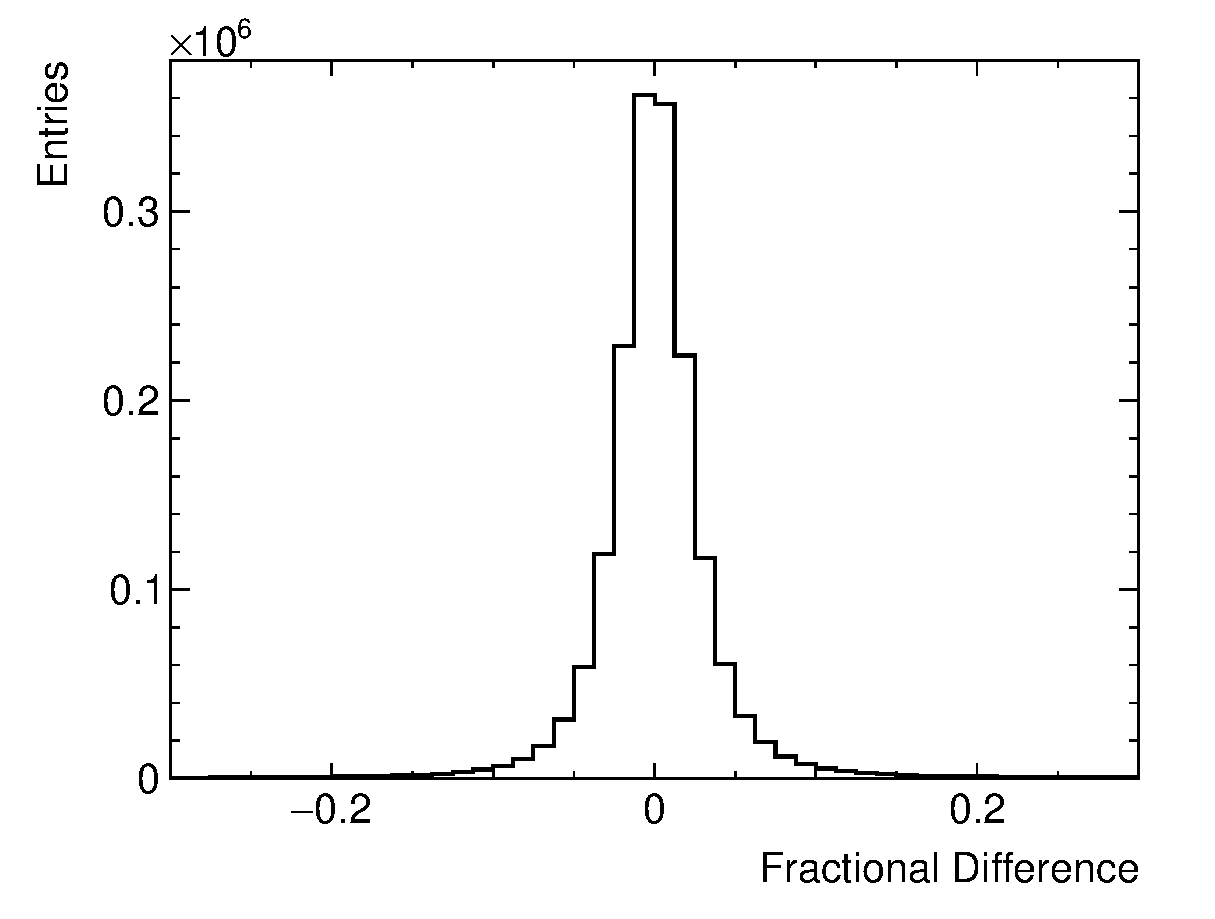
\includegraphics[width=\sgfigwid\textwidth]{figures/tuning/residual.eps}
    \caption{\label{fig:residual} Fractional difference for the bin-by-bin cross sections between MC truth and the parametrised approximation using fourth-order polynomials, both in the Norm-Shape (NS)~\cite{DAgostini:1993arp,Hanson:2005mrg} space with \allpar. See Table~\ref{tab:restunes} for the definition of \allpar. The residual exhibits a mean of $0.003$ and a standard deviation of $0.073$.} 
\end{figure}

Furthermore, to circumvent Peelle's Pertinent Puzzle\footnote{This is a phenomenon where unknown correlations between observables can skew the $\chi^2$ minimisation.}~\cite{PPP_FNL,Chakrani:2023htw}, the Norm-Shape (NS) transformation prescription~\cite{DAgostini:1993arp,Hanson:2005mrg} is adopted. 
Thereafter, the extremal point is determined by minimizing $\chi^2$ between the NS-transformed polynomial approximation and the NS-transformed data. 
During the minimisation process, priors—typically derived from systematic uncertainties—are imposed on each parameter to prevent them from deviating excessively from their nominal values. 
The following subsections elaborate on the specific measurement observables and model parameters to be tuned.

\section{Inputs}
The first step towards tuning is to identify the models to be tuned and the data to be used by spotting the lacking area of the current model, which is manifested by the data-MC discrepancy.
One such example is illustrated in Fig.~\ref{fig:g24-0-dat-reac} and Fig.~\ref{fig:g24-0-pn-reac}, which shows the data-MC comparison using \newtune, one of the latest Comprehensive Model Configurations (CMC) in \genie, for four TKI measurements, namely \ttkzpi~\cite{T2K:2018rnz}, \ttkpip~\cite{T2K:2021naz}, \minzpi~\cite{MINERvA:2018hba, MINERvA:2019ope}, and \minpiz~\cite{MINERvA:2020anu}. 
\begin{figure*} 
    \centering 		
    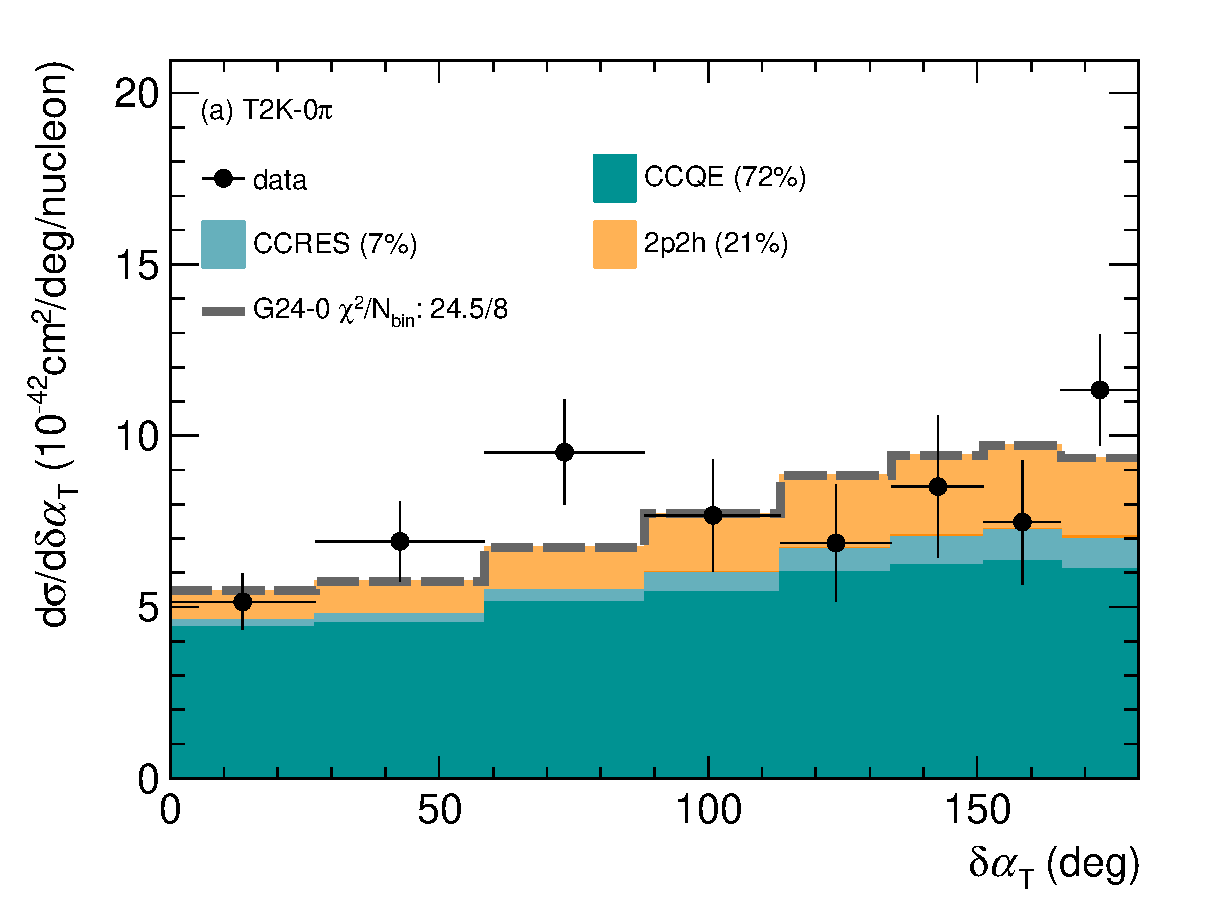
\includegraphics[width=\dbfigwid\textwidth]{figures/tuning/0000-t2k_0pi_dalphat_reac_decomp.eps} 
    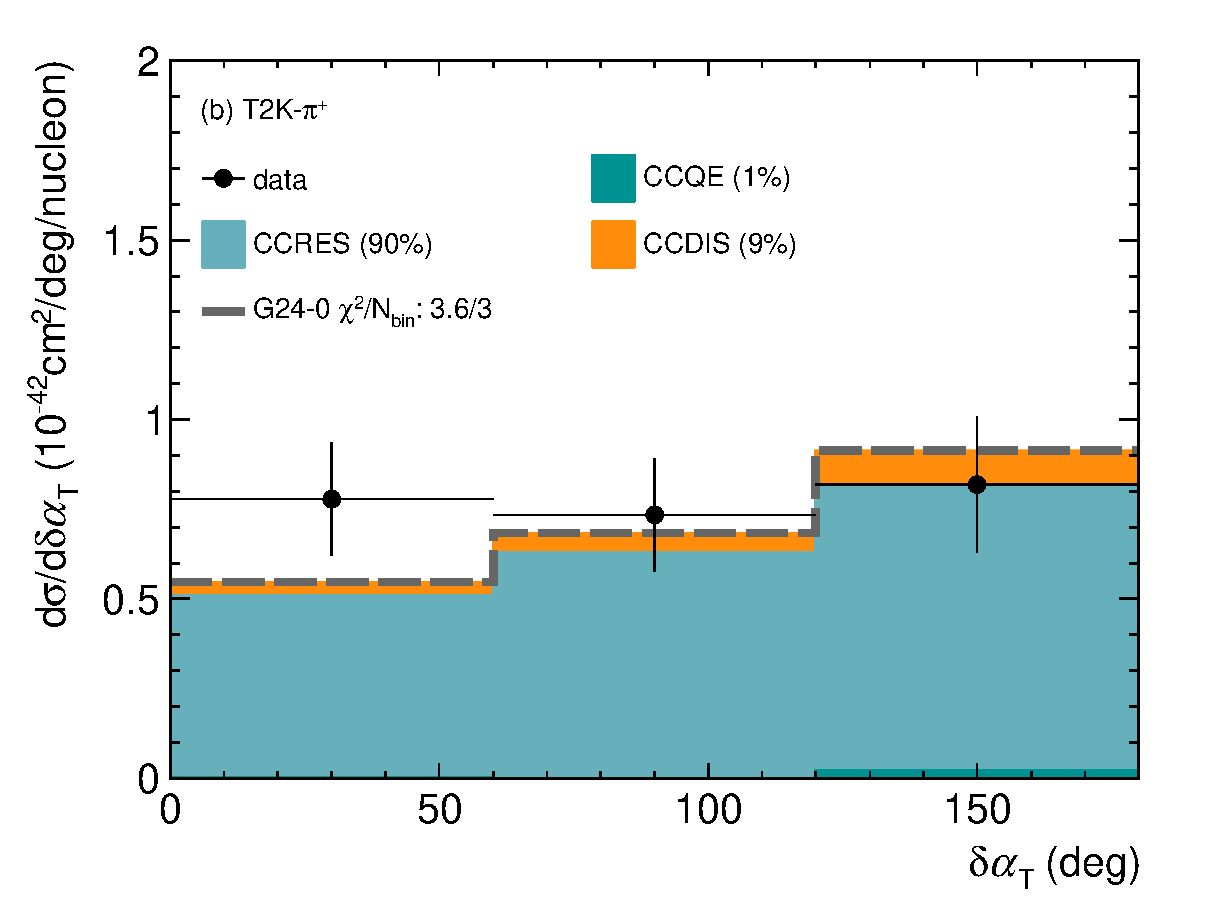
\includegraphics[width=\dbfigwid\textwidth]{figures/tuning/0000-t2k_pip_dalphat_reac_decomp.eps} 
    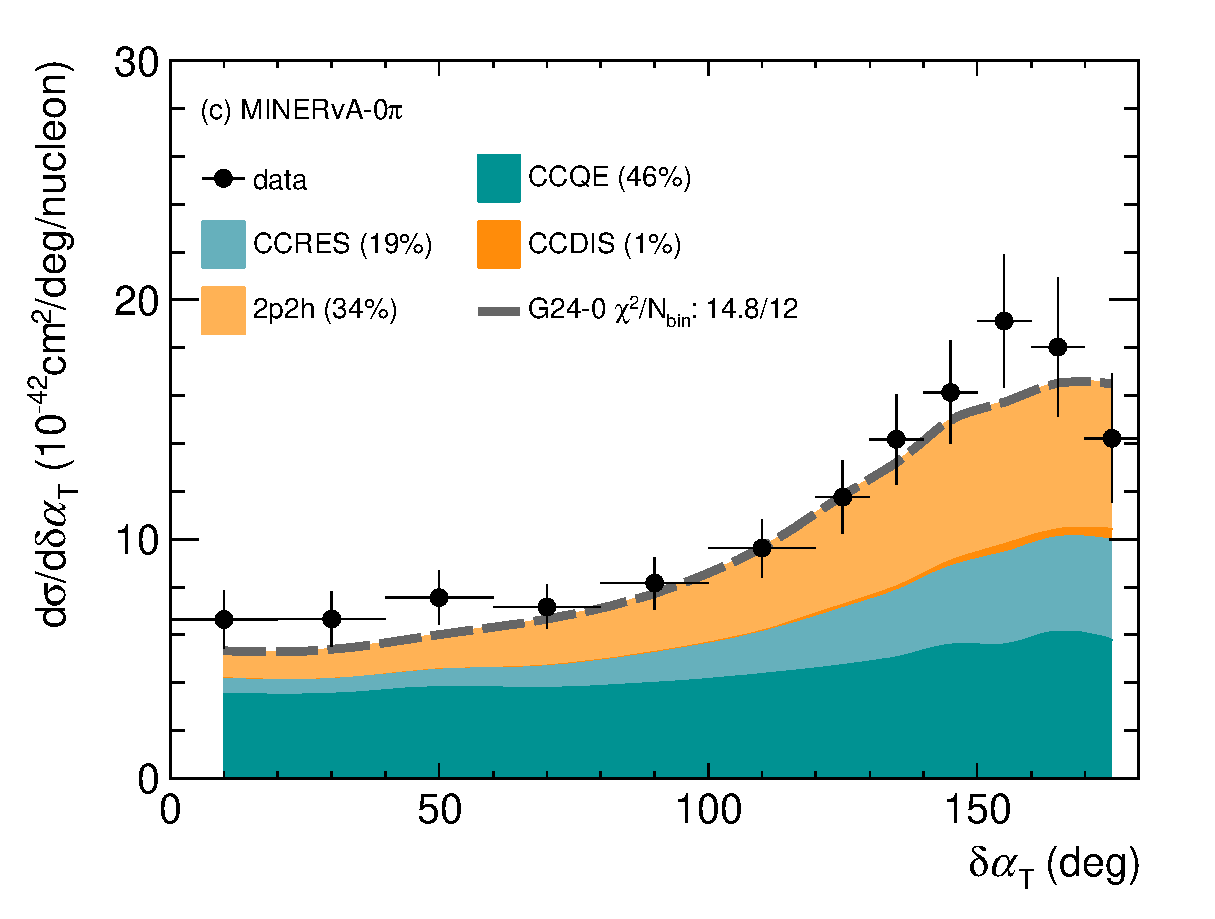
\includegraphics[width=\dbfigwid\textwidth]{figures/tuning/0000-min_0pi_dalphat_reac_decomp.eps} 
    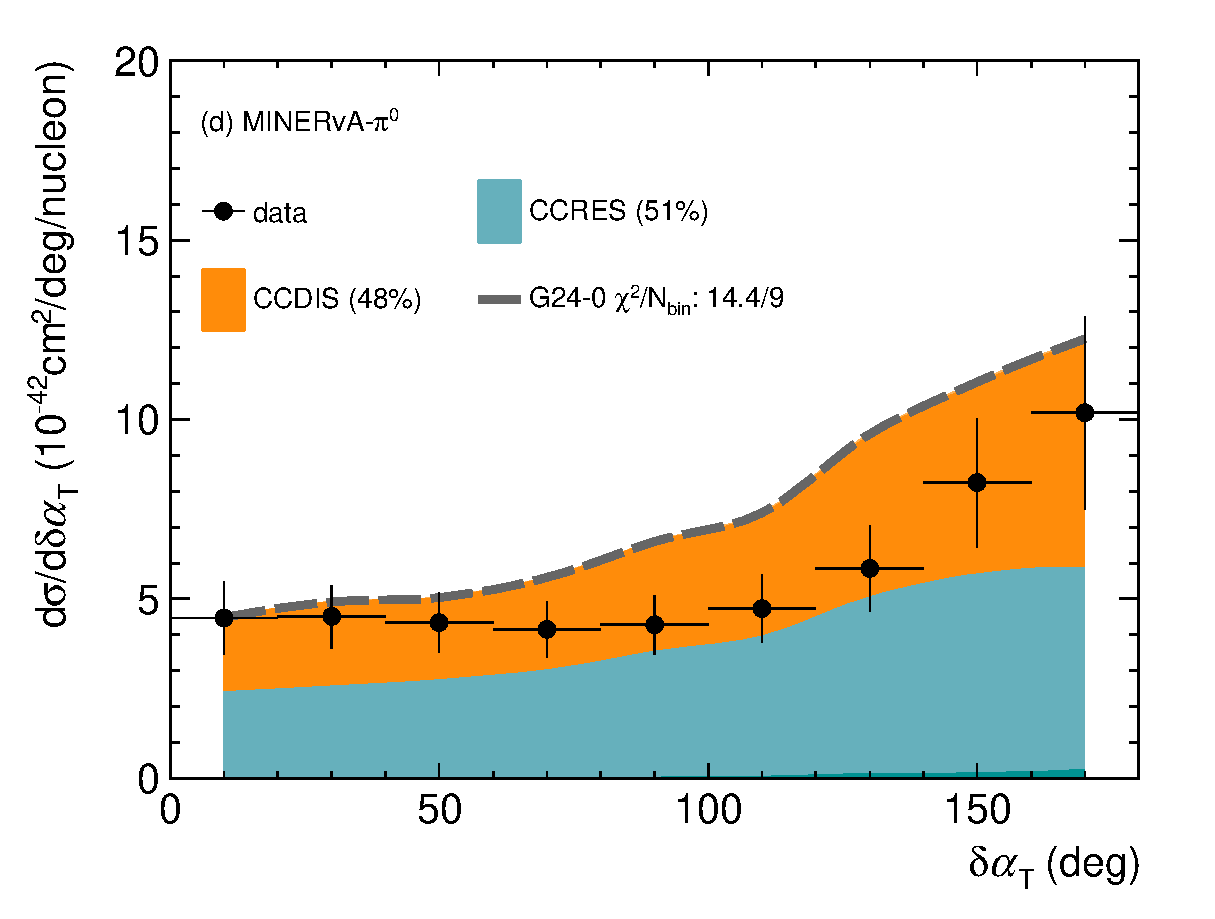
\includegraphics[width=\dbfigwid\textwidth]{figures/tuning/0000-min_pi0_dalphat_reac_decomp.eps}
    \caption{$\dat$ measurements decomposed in interaction types, compared to \gZero\ prediction.}   \label{fig:g24-0-dat-reac} 
            
    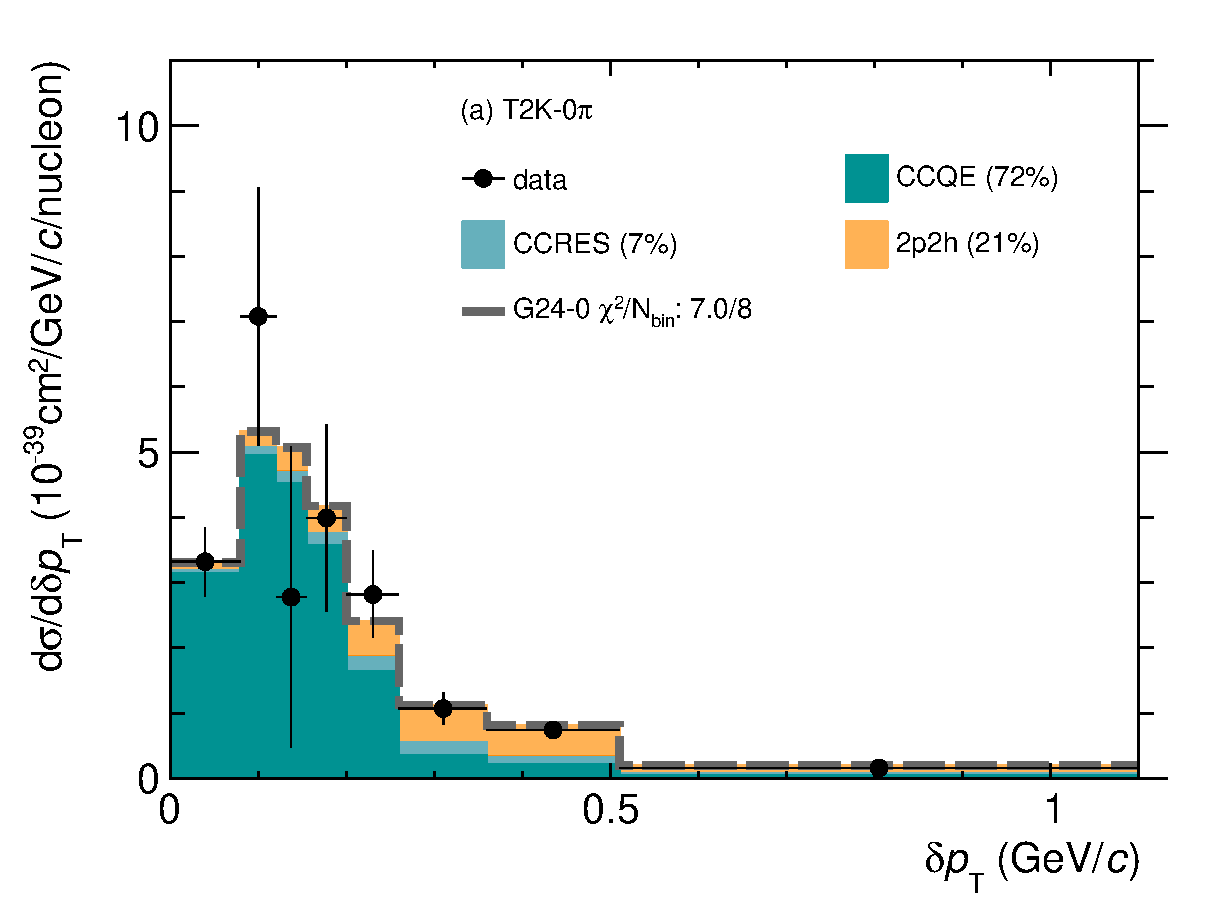
\includegraphics[width=\dbfigwid\textwidth]{figures/tuning/0000-t2k_0pi_dpt_reac_decomp.eps}
    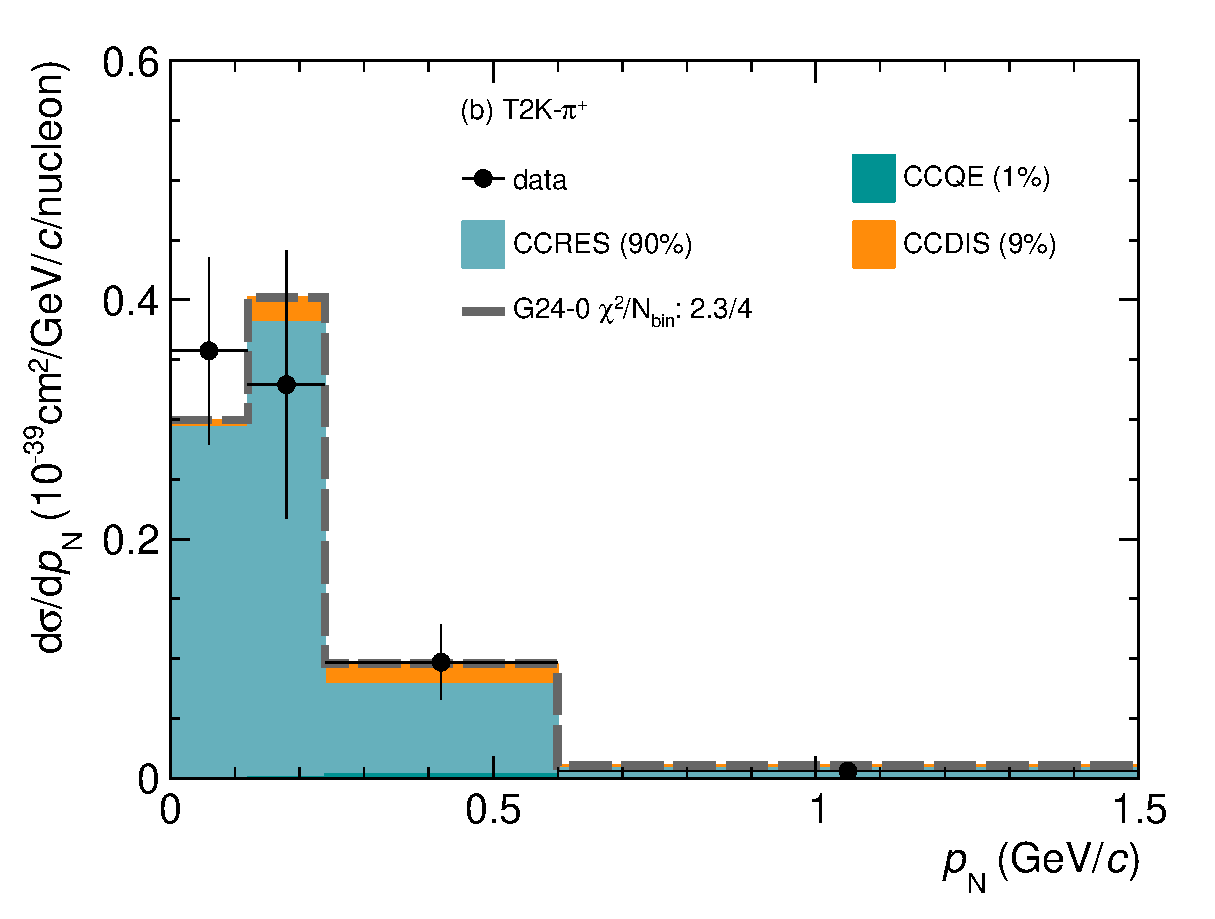
\includegraphics[width=\dbfigwid\textwidth]{figures/tuning/0000-t2k_pip_pn_reac_decomp.eps}
    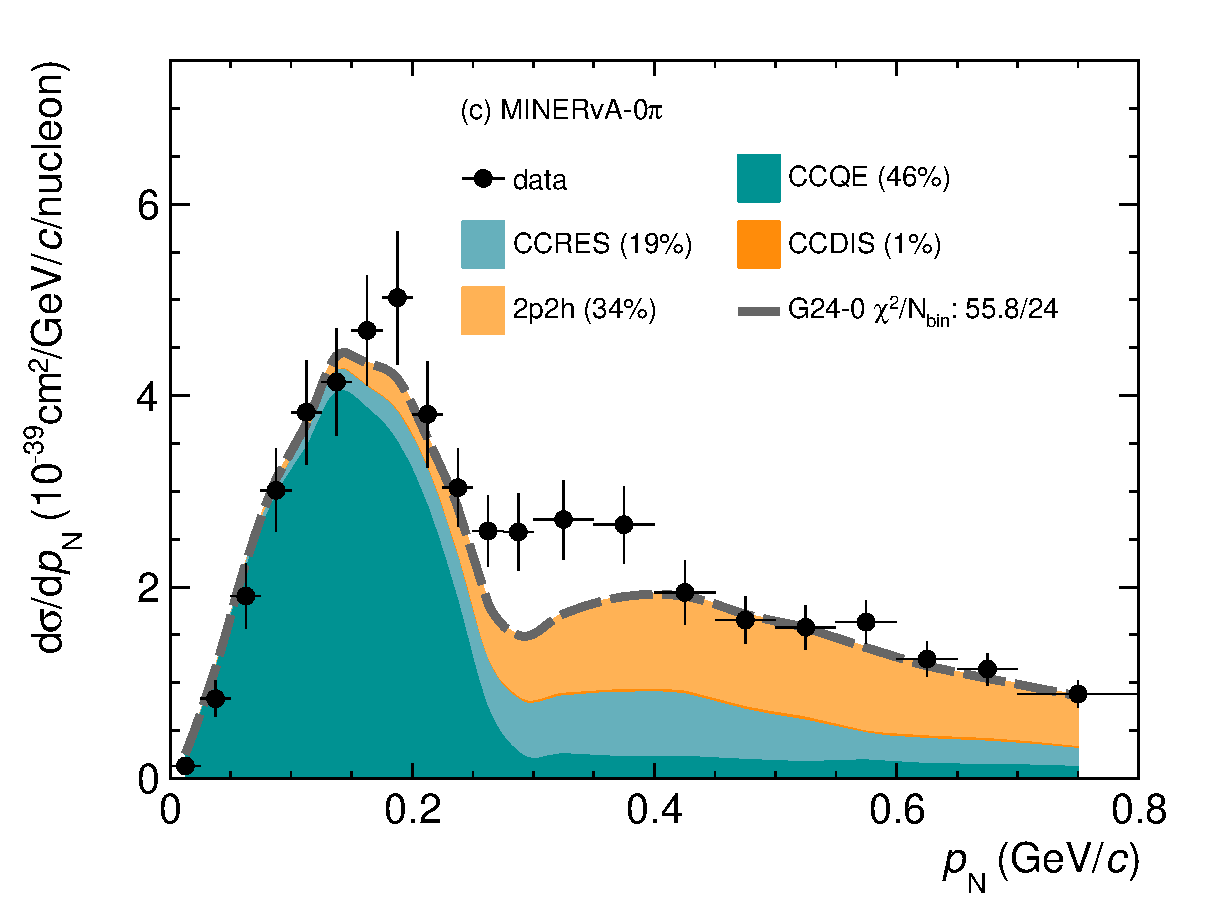
\includegraphics[width=\dbfigwid\textwidth]{figures/tuning/0000-min_0pi_pn_reac_decomp.eps}
    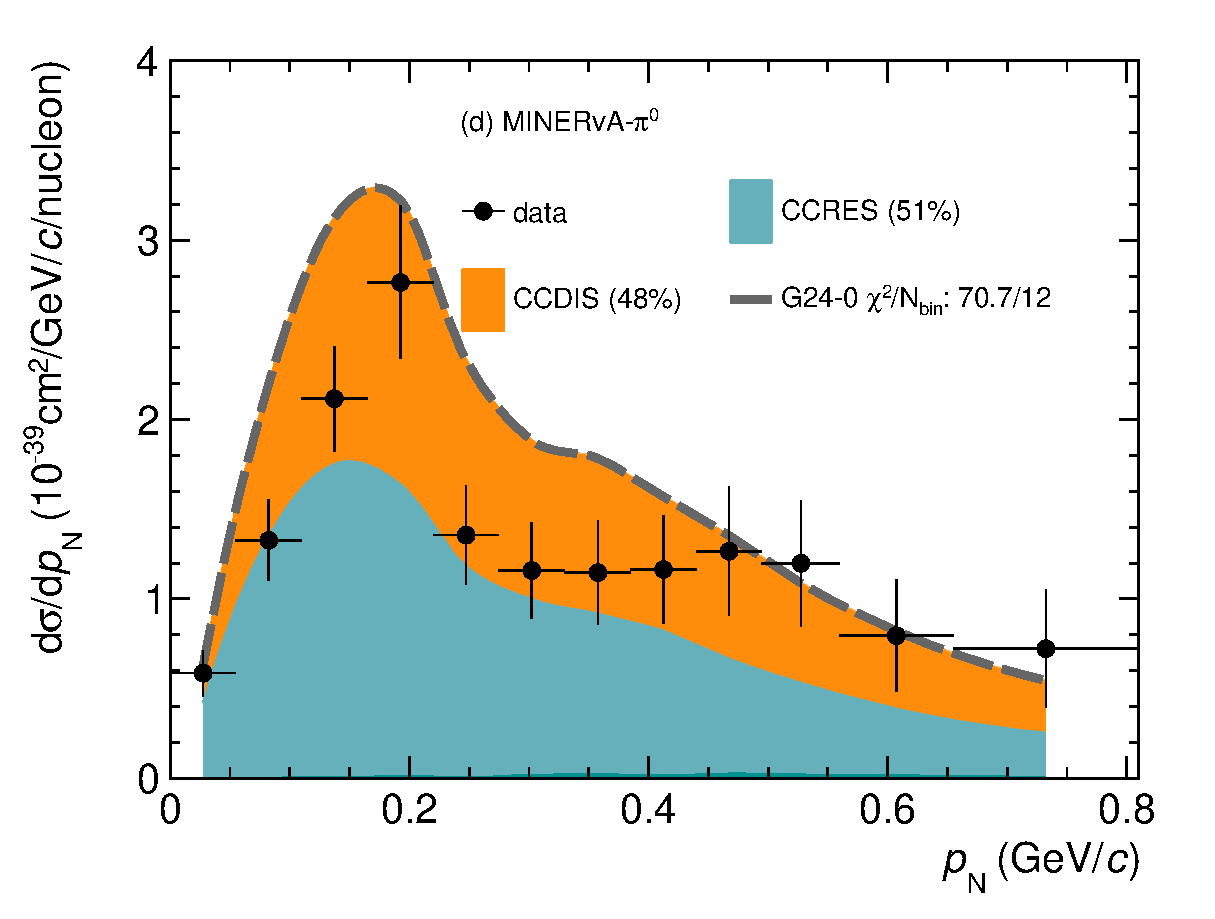
\includegraphics[width=\dbfigwid\textwidth]{figures/tuning/0000-min_pi0_pn_reac_decomp.eps}
    \caption{\label{fig:g24-0-pn-reac} Similar to Fig.~\ref{fig:g24-0-dat-reac} but for the $\pn$ (\ttkpip, \minzpi, and \minpiz) and $\dpt$ (\ttkzpi) measurements.
    } 
\end{figure*}
This data-comparison shows that the model fails to describe the MINERvA $\piz$ TKI data, despite that its prediction matches other TKI data well.

As the neutrino-nucleus interaction is a complicated process, it requires multiple models to simulate the whole process, and the CMC in \genie\ specifies the combination of models to be used.
Tuning the entire CMC is extremely computationally expensive, and this is the first tuning on TKI data across event topology, i.e. on both $\cczpi$ and $\ccopi$. 
Hence, before embarking on this ultimate step, it is important to first perform a proof-of-concept study to explore the model flexibility and to identify the most relevant model parameters.
As TKI data are sensitive to the nuclear IS and FSI, this study focuses on the tuning of these two models.
To lay the ground for better understanding of this tuning effort, I will provide a more detailed description of the inputs, i.e. the data and the models, in the following subsections. 

\subsection{The models}
\label{sec:tuning-para-choice}
    The CMCs in \genie\ are formatted strings, and they are sometimes also called tunes, regardless of whether they are obtained from an actual tuning.
    The tune, \newtune, mentioned above is improved on the tune, $\geighteen$, which is obtained from the free nucleon tuning effort in Ref.~\cite{GENIE:2021zuu}, and describes bubble chamber data better.
    As \newtune\ is widely used in the paper, it will be referred to as \gZero\ for simplicity. 

    The IS in \gZero\ is modelled by the spectral-function-like Correlated Fermi Gas model (\sfcfg)~\cite{sfcfg-talk,sfcfg-GitHubCommit,GENIE:2021npt}. 
    \sfcfg\ has more adjustable parameters for tuning and improved physics compared to the local fermi gas (LFG) model used in $\geighteen$.
    The improvement arises from two aspects. 
    ``Spectral-function-like'' refers to the implementation of removal energy as a varying function rather than a fixed value, while ``Correlated'' highlights the incorporation of the high-momentum tail above the Fermi momentum due to nucleon-nucleon short-range correlations (SRC), as evidenced by electron-scattering data~\cite{CLAS:2005ola}.

    Both enhancements are incorporated into the Valencia Model~\cite{Nieves:2004wx}).  
    Consequently, \sfcfg\ more closely reproduces the Valencia initial state than previous LFG implementations.  
    For further details on \sfcfg, see Ref.~\cite{GENIE:2021npt}.  
    Note that the original Valencia Model employs its own approach to modelling FSI. 
    However, since FSI is factorized from other processes in the \genie\ implementation, that method is not applied here.  
    Instead, GENIE has developed the INTRANUKE hA FSI model (hA for short), which is chosen as the FSI candidate for the tuning performed in this work for its simplicity and interpretability.

    Additional improvements of \gZero\ include:  
    1) adopting a $z$-expansion axial-vector form factor~\cite{Hill:2010yb} in lieu of the Valencia dipole form factor for QE processes~\cite{Nieves:2004wx}; and  
    2) substituting the Valencia model for 2p2h processes~\cite{Nieves:2011pp} with the SuSAv2 Model~\cite{Gonzalez-Jimenez:2014eqa}, which covers a broader region of the $q^0$ and $q^3$ phase space.  
    The complete list of model components is provided in Table~\ref{tab:default-gen-list}.
    \begin{table}[!htb]
        \centering
        \begin{tabular}{p{4cm}c}
        \hline
        \hline
        \textrm{Simulation component} & \textrm{Model} \\
        \hline
        \textrm{Nuclear state}              & \sfcfg~\cite{sfcfg-talk,sfcfg-GitHubCommit,GENIE:2021npt} \\ 
        \textrm{QE}               & Valencia~\cite{Nieves:2004wx} \\
        \textrm{2p2h}               & SuSAv2~\cite{Gonzalez-Jimenez:2014eqa} \\
        \textrm{QE $\Delta S=1$}           & Pais~\cite{Pais:1971er} \\
        \textrm{QE $\Delta C=1$}                  & Kovalenko~\cite{Kovalenko:1990zi} \\
        \textrm{Resonance (RES)}                        & Berger-Sehgal~\cite{Berger:2007rq}\\
        Shallow/Deep inelastic \par scattering (SIS/DIS)                    & Bodek-Yang~\cite{Bodek:2002vp}\\
        \textrm{DIS $\Delta C=1$}           & Aivazis-Tung-Olness~\cite{Aivazis:1991fy}\\
        \textrm{Coherent $\pi$ production}  & Berger-Sehgal~\cite{Berger:2008xs}\\
        \hline
        \textrm{Hadronization}              & AGKY~\cite{Yang:2009zx}\\
        \textrm{FSI}                        & INTRANUKE hA~\cite{Andreopoulos:2015wxa}\\
        \hline
        \hline
        \end{tabular}
        \caption{\label{tab:default-gen-list} Model components of \gZero. Processes with non-trivial $\Delta S$ and $\Delta C$ are those with strangeness and charm production, respectively.}
    \end{table}
    Having selected the \gZero\ CMC as the tuning starting point, a closer look into the IS and FSI models, the models to be tuned, is necessary.
    The \sfcfg\ and hA model contains a total of $14$ tuneable parameters of \sfcfg\ and hA.

    The \sfcfg\ model behaviour is chiefly specified by two parameters: 
    $\srcfr$, which quantifies the fraction of the high-momentum tail from SRC above the Fermi surface, and 
    $\nurmec$, which defines the onset of the nuclear removal energy distribution for carbon.  
    A higher $\srcfr$ suggests that the initial nucleons possess greater energy, whereas a larger $\nurmec$ implies that more energy is required to liberate a nucleon, resulting in lower-energy final-state particles.  
    Due to the innovative yet loosely constrained nature of this spectral-function-like implementation, this study adopts relatively lenient priors of \(0.12\pm0.12\) for $\srcfr$ and \(0.01\pm0.005~\gev\) for $\nurmec$.

    As for the hA model~\cite{Andreopoulos:2015wxa}, its widespread use is primarily due to its straightforward reweighting capability. 
    Unlike cascade models such as the hN model~\cite{Andreopoulos:2015wxa}, the hA model assigns the FSI type for each hadron exactly once, without simulating further propagation of rescattered hadrons. 
    This single-rescattering approach is critical for interpreting tuning results. The hA model parameters are described as follows.
    \begin{enumerate}
        \item \textbf{Mean Free Path (MFP) Scaling Factors}:
        The model computes the MFP, $\lambda$, as a function of the hadron's energy, $E$, and its radial distance, $r$, from the nucleus centre:
        \begin{equation}
            \lambda(E,r) = \frac{1}{\sigma_\textrm{hN,tot}(E)\rho(r)},
        \end{equation}
        where $\sigma_\textrm{hN,tot}$ is the total hadron–nucleon cross section and $\rho(r)$ is the local nucleon density. 
        Once produced within the nucleus, a hadron travels a distance $\lambda$ before a probabilistic decision on rescattering is made. 
        If no rescattering occurs, the hadron is propagated by another $\lambda$, and the process repeats until either a rescattering happens or the hadron escapes the nucleus. 
        When rescattering occurs, its type is chosen based on the relevant cross sections; the relative probabilities of these types are extracted from stored hadron scattering data~\cite{LADS:1999dyv,Navon:1983xj,Carroll:1976hj,Clough:1974qt,BAUHOFF1986429,Mashnik:2000up,Ishibashi:1997gbe}. 
        Once a specific rescattering type is determined, the resulting products are generated and considered final, with no further rescattering simulated.
        The MFPs for pions and nucleons are adjustable via scaling factors ($\cpimfp$, $\pizmfp$, and $\nmfp$) as detailed in Table~\ref{tab:restunes}. 
        Due to isospin symmetry, both charged pions, $\pip$ and $\pim$, share the same scaling factor $\cpimfp$, while the $\piz$ MFP is computed from the charged pion values and adjusted separately by $\pizmfp$. 
        A scaling factor greater than unity increases $\lambda$, which in turn reduces the number of propagation steps necessary for escape and diminishes the average probability of rescattering. 
        Owing to the high precision of total hadron–nucleus cross section measurements~\cite{LADS:1999dyv,Navon:1983xj,Carroll:1976hj,Clough:1974qt,BAUHOFF1986429}, strict Gaussian priors with a standard deviation ($\sigma$) of 0.2 (matching the systematic uncertainties shown in Table~\ref{tab:restunes}) are applied to the MFP scaling factors. 
        Notably, varying $\pizmfp$ by $\pm2.5~\sigma$ significantly affects the \minpiz\ $\textrm{d}\sigma/\textrm{d}\pn$, as illustrated in Fig.~\ref{fig:minpiz-pn-pi0mfp}. 
        In summary, a reduced MFP naturally increases rescattering, leading to fewer $\piz$s escaping the nucleus and a decreased cross section.
        \begin{figure}[!htb]
            \centering
            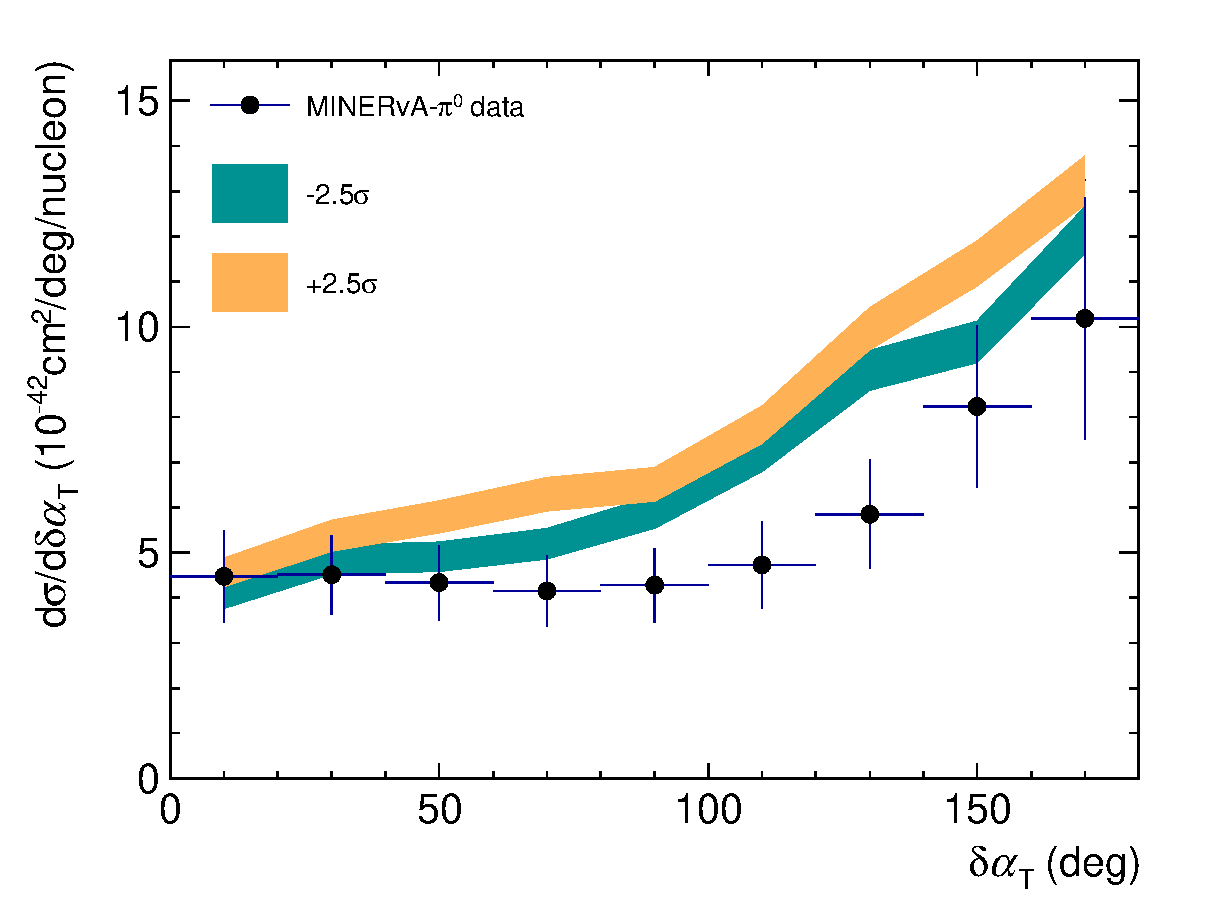
\includegraphics[width=\sgfigwid\textwidth]{figures/tuning/minerva_pi0_dalphat_FSI_pi0mfp.eps}
            \caption{Effect of varying $\pizmfp$ by $\pm2.5~\sigma$ compared to the MINERvA-$\pi^0$ measurement. Each band's width indicates the \genie\ prediction's statistical uncertainty from $10^5$ events.}
            \label{fig:minpiz-pn-pi0mfp}
        \end{figure}

        \item \textbf{Rescattering Type Scaling Factors}: 
        The relative probability for each rescattering type is adjusted by a scaling factor. 
        Four rescattering types are available for both nucleons and pions: charge exchange (CEX), inelastic scattering (INEL), absorption (ABS), and pion production (PIPD). 
        A detailed discussion of these tunable FSI types is provided in Sec.~\ref{sec:nuint-fsi}. 
        The default energy-dependent probability distributions, derived from hadron data tuning~\cite{LADS:1999dyv,Navon:1983xj,Carroll:1976hj,Clough:1974qt,BAUHOFF1986429}, are modified by corresponding scaling factors (e.g., $\picex$ for the CEX of all pions) as listed in Table~\ref{tab:restunes}. 
        After scaling, the probabilities are renormalized so that they sum to one. 
        For instance, if the initial absorption fraction, $f_\textrm{ABS}$, is 0.5 (with the remaining fraction, $f_\textrm{other}=f_\textrm{INEL}+f_\textrm{CEX}+f_\textrm{PIPD}$, also 0.5), scaling $f_\textrm{ABS}$ by $S_\textrm{ABS}=2$ yields
        \begin{equation}
            f^\prime_\textrm{ABS} = \frac{f_\textrm{ABS} \cdot S_\textrm{ABS}}{f_\textrm{ABS} \cdot S_\textrm{ABS}+f_\textrm{other}} = \frac{2}{3},
        \end{equation}
        illustrating that the effective increase in $f_\textrm{ABS}$ is less than the scaling factor alone due to normalization with the other FSI types.
        Here, $f_\textrm{ABS}$ is effectively scaled by a factor of 1.3 rather than 2. 
        Therefore, a relatively relaxed Gaussian prior with a $\sigma$ of 0.5 is imposed on the FSI fate scales, slightly exceeding the systematic uncertainties in Table~\ref{tab:restunes}.
        A side-effect due to this normalization is that changing one scaling factor inherently affects the others.
        In practice, plotting the cross section by rescattering type clarifies the net changes.
    \end{enumerate}
    
    Table~\ref{tab:restunes} summarizes the tuneable parameters and their ranges imposed in tuning.
    Nominal values and associated uncertainties for the hA model are taken from Table 17.3 in Ref.~\cite{Andreopoulos:2015wxa}. 
    \begin{table}[!htb]
        \centering
        \begin{tabular}{ccccc}
        \hline
        \hline
        Parameter & Nominal (\gZero) & Range In Tuning & \redpar (\gC) & \allpar (\gT) \\
        \hline
        \multicolumn{5}{c}{\sfcfg} \\
        \hline
        $\srcfr$  & 0.12          & (0.0, 0.5)  & 0.09 $\pm$ 0.08         & 0.17 $\pm$ 0.10       \\
        $\nurmec$ & 0.01          & (0.0, 0.2)  & 0.01                    & 0.06 $\pm$ 0.000004     \\
        \hline
        \multicolumn{5}{c}{hA} \\
        \hline
        $\cpimfp$ & $1.0\pm0.2$   & (0.0, 3.0)  & 1.0                     & 1.21 $\pm$ 0.15         \\
        $\pizmfp$ & $1.0\pm0.2$   & (0.0, 3.0)  & 0.34 $\pm$ 0.11         & 0.91 $\pm$ 0.000004     \\
        $\nmfp$   & $1.0\pm0.2$   & (0.0, 3.0)  & 1.0                     & 0.89 $\pm$ 0.000382     \\
        \hline
        $\picex$  & $1.0\pm0.5$   & (0.0, 3.0)  & 0.27 $\pm$ 0.28         & 0.86 $\pm$ 0.000056      \\
        $\ncex$   & $1.0\pm0.5$   & (0.0, 3.0)  & 1.39 $\pm$ 0.33         & 0.92 $\pm$ 0.001178       \\
        \hline
        $\piinel$ & $1.0\pm0.4$   & (0.0, 3.0)  & 1.0                     & 0.90 $\pm$ 0.00008       \\
        $\ninel$  & $1.0\pm0.4$   & (0.0, 3.0)  & 1.0                     & 0.92 $\pm$ 0.001218       \\
        \hline
        $\cpiabs$ & $1.0\pm0.2$   & (0.0, 3.0)  & 1.0                     & 1.36 $\pm$ 0.38          \\
        $\pizabs$ & $1.0\pm0.2$   & (0.0, 3.0)  & 1.0                     & 0.92 $\pm$ 0.000024     \\
        $\nabs$   & $1.0\pm0.2$   & (0.0, 3.0)  & 0.48 $\pm$ 0.33         & 1.02 $\pm$ 0.413668      \\
        \hline
        $\pipiprod$ & $1.0\pm0.2$ & (0.0, 3.0)  & 1.0                     & 1.11 $\pm$ 0.342484       \\
        $\npiprod$  & $1.0\pm0.2$ & (0.0, 3.0)  & 1.90 $\pm$ 0.71         & 1.12 $\pm$ 0.57198        \\ 
        \hline
        \hline
        \multicolumn{5}{c}{$\chi^2$ for \texttt{combi}} \\
        \hline
        &\texttt{untuned}    &  & 231.75         & 129.61        \\
        &\texttt{tuned}      &  & 168.67         & 131.46        \\
        &\texttt{diff}       &  & -63.08         & 1.85         \\
        \hline
        \multicolumn{5}{c}{$\chi^2$ for \texttt{vald}} \\
        \hline
        &\texttt{untuned}    &  & 229.5          & 331.64        \\
        &\texttt{tuned}      &  & 232.3          & 304.4         \\
        &\texttt{diff}       &  & 2.8            & -27.24        \\
        \hline
        \multicolumn{5}{c}{$\chi^2$ for \texttt{combi+vald}} \\
        \hline
        &\texttt{untuned}    &  & 461.25         & 461.25        \\
        &\texttt{tuned}      &  & 400.97         & 435.86        \\
        &\texttt{diff}       &  & -60.28         & -25.39  \\     
        \hline
        \hline
        \end{tabular}
        \caption{\label{tab:restunes}
            Parameters in \gZero, \gC, and \gT. Lower section: \texttt{combi} indicates that the following $\chi^2$ sums are calculated for the tuned measurements, while \texttt{vald} indicates that the respective validation sets are used; \texttt{untuned} means that the $\chi^2$ calculation uses the nominal values of the parameters, while \texttt{tuned} denotes the tuned ones. \texttt{diff} displays the improvement achieved by the respective tuning.
        }
    \end{table}

    % \begin{table}[!htb]
    %     \centering
    %     \begin{tabular}{ccccc}
    %     \hline
    %     \hline
    %     \textrm{Parameter} & \textrm{Nominal} (\gZero)     & \textrm{Range In} \textrm{Tuning} & \allpar (\gT)  & \redpar (\gC) \\ 
    %     \hline
    %     \multicolumn{5}{c}{\sfcfg} \\
    %     \hline
    %     \textrm{$\srcfr$} & 0.12 & (0.0, 0.5)  & \tick & \tick\\
    %     \textrm{$\nurmec$} & 0.01 & (0.0, 0.2) & \tick & \\
    %     \hline
    %     \multicolumn{5}{c}{hA} \\
    %     \hline
    %     \textrm{$\cpimfp$} & $1.0\pm0.2$ & (0.0, 3.0) & \tick & \\
    %     \textrm{$\pizmfp$} & $1.0\pm0.2$ & (0.0, 3.0) & \tick & \tick\\
    %     \textrm{$\nmfp$} & $1.0\pm0.2$ & (0.0, 3.0) & \tick &\\
    %     \hline
    %     \textrm{$\picex$} &  $1.0\pm0.5$ & (0.0, 3.0) & \tick & \tick \\
    %     \textrm{$\ncex$} & $1.0\pm0.5$ & (0.0, 3.0)  & \tick & \tick\\
    %     \hline
    %     \textrm{$\piinel$} & $1.0\pm0.4$ & (0.0, 3.0) & \tick & \\
    %     \textrm{$\ninel$} & $1.0\pm0.4$ & (0.0, 3.0)  & \tick &\\
    %     \hline
    %     \textrm{$\cpiabs$} & $1.0\pm0.2$ & (0.0, 3.0) & \tick &\\
    %     \textrm{$\pizabs$} & $1.0\pm0.2$ & (0.0, 3.0) & \tick &\\
    %     \textrm{$\nabs$} & $1.0\pm0.2$ & (0.0, 3.0)  & \tick & \tick\\
    %     \hline
    %     \textrm{$\pipiprod$} & $1.0\pm0.2$ & (0.0, 3.0) & \tick &\\
    %     \textrm{$\npiprod$} & $1.0\pm0.2$ & (0.0, 3.0)  & \tick & \tick\\
    %     \hline
    %     \hline
    %     \end{tabular}
    %     \caption{\label{tab:hALFG-para}
    %     Tuneable parameters and their ranges in the  \sfcfg\ (\textit{uppermost} group) and hA (\textit{lower} groups, uncertainties from Ref.~\cite{Andreopoulos:2015wxa}) models. Parameters to be tuned in the two sets are marked with ``\tick'''s. See later text for definitions of \gT and \gC.
    %     }
    % \end{table}

\subsection{The data}
    Not only the \minpiz\ data set, where the discrepancy lies, is used for tuning, but the other three data sets are also included, as it is important to maintain the good data-MC agreement for the existing data sets, while improving the agreement for the \minpiz\ data set.

    The common requirement of the four measurements is the presence of one CC muon and at least one proton in the final state. 
    The $0\pi$ data sets, i.e. \ttkzpi\ and \minzpi, require the absence of any pions, while \ttkpip\ requires exactly one $\pi^+$, and \minpiz\ requires at least one $\pi^0$.
    The four data sets further differ slightly in the kinematic cuts, as summarized in Table~\ref{tab:fit-var-combo-phase-space-cut}, and they also contain slightly different combinations of the TKI variables, as detailed in Table~\ref{tab:fit-var-combo}.
    \begin{table}[!htb]
        \centering
        \begin{tabular}{cc}
        \hline
        \hline
        Variables & Cuts ($p$ in $\gevc$) \\
        \hline
        \multicolumn{2}{c}{\ttkzpi~\cite{T2K:2018rnz}} \\
        \hline
        $\vecpmu$    &  $0.25 < p_\mu $, $\cos\theta_\mu>-0.6$   \\
        $\vecpp$     & $0.45< p_\text{p} <1.0$ , $\cos\theta_\text{p}>0.4$     \\
        \hline
        \multicolumn{2}{c}{\ttkpip~\cite{T2K:2021naz}} \\
        \hline
        $\vecpmu$    & $0.25 < p_\mu < 7$ , $\theta_\mu < 70^\circ$  \\
        $\vecpp$     & $0.45 < p_\text{p} <1.2$  ,  $\theta_\text{p} < 70^\circ$   \\
        $\vecppi$    & $0.15 < p_\pi <  1.2$, $\theta_\pi < 70^\circ$ \\
        \hline
        \multicolumn{2}{c}{\minzpi~\cite{MINERvA:2018hba, MINERvA:2019ope}} \\
        \hline
        $\vecpmu$     & $1.5< p_\mu < 10$ , $\theta_\mu < 20^\circ $  \\
        $\vecpp$      & $0.45< p_\text{p} <1.2$  , $\theta_\text{p} < 70^\circ$    \\
        \hline
        \multicolumn{2}{c}{\minpiz~\cite{MINERvA:2020anu}} \\
        \hline
        $\vecpmu$   & $1.5< p_\mu < 20$ , $\theta_\mu < 25^\circ$  \\
        $\vecpp$    & $0.45< p_\text{p} $                      \\
        \hline
        \hline
        \end{tabular}
        % \end{ruledtabular}
        \caption{\label{tab:fit-var-combo-phase-space-cut}
        Kinematic cuts for the samples of the TKI measurements.
        }
    \end{table}

    As not all TKI observables are linearly independent, such as $\dpt$ and $\pn$, and some might have strong dependence outside IS and FSI, such as $\dphit$ displaying a strong dependence on neutrino beam energy~\cite{Lu:2015tcr}, it might be redundant and ineffective to include all of them in the tuning.
    In order to discern the most sensitive observables, a systematic evaluation of various combinations of observables was undertaken for the tuning process. 
    A total of 26 combinations, as shown in Table~\ref{tab:fit-var-combo}, are examined. 
    These combinations are formed according to the following patterns:
    \begin{itemize}
        \item \textbf{\texttt{Combi-}1 through 5} are cross-experiment selections of a single observable. 
        For example, \texttt{Combi-}$3$ uses only $\dat$ from all four data sets. 
        If a chosen observable is absent from a dataset, that dataset is excluded from the specific combination. 
        For example, \ttkzpi\ is not used in \texttt{Combi-}1 due to the absence of $\pn$.
        \item \textbf{\texttt{Combi-}6 through 9} incorporate all variables from a single measurement. For example, \texttt{Combi-}$9$ uses \minpiz\ only.
        \item \textbf{\texttt{Combi-}10 to 13} uses two out of four measurements according to the experiment or topology. For example, \texttt{Combi-}$10$ uses only the two data sets from T2K, and \texttt{Combi-}$13$  only with pion production. 
        \item \textbf{\texttt{Combi-}14 to 17} are cross-experiment selections of two observables. 
        For example, \texttt{Combi-14} uses all $\dat$ and $\dptt$ measurements across all data sets, while \texttt{Combi-17} uses $\dat$ and $\dpt$.
        \item \textbf{\texttt{Combi-}18 through 22} are cross-experiment selections of three observables. 
        For example, \texttt{Combi-18} uses all available $\dat$, $\dptt$, and $\pn$, while \texttt{Combi-22} uses $\dpt$, $\dphit$, and $\pn$.
        \item \textbf{\texttt{Combi-}23} uses all observables except $\dphit$ from all data sets.
        \item \textbf{\texttt{Combi-}24} encompasses all variables, acting as the superset.
        \item \textbf{\texttt{Combi-}25 and 26} are the same as \texttt{Combi-}$21$ and $23$, respectively, except that $\dpt$ in \minzpi\ is removed to avoid correlation with $\pn$ in the same data set.
    \end{itemize}

    \begin{table}[h]
    \centering
    \resizebox{\textwidth}{!}{%
    \begin{tabular}{c|c|ccccc|cccc|cccc|cccc|ccccc|c|c|cc}
    \hline
    \hline
    \texttt{Combi-} & $\#$ of bins & 1 & 2 & 3 & 4 & 5 & 6 & 7 & 8 & 9 & 10 & 11 & 12 & 13 & 14 & $15^{*}$  & 16 & 17 & 18 & 19 & 20 & 21 & 22 & 23 & 24  & 25 & 26^{\dagger}\\
    \hline
    \multicolumn{27}{c}{\ttkzpi} \\
    \hline
    $\dat$    & 8  &   &   & $\tick$ &   &   & $\tick$ &   &   &   & $\tick$  &    & $\tick$  &    & $\tick$  &    & $\tick$  & $\tick$  & $\tick$  & $\tick$  & $\tick$  & $\tick$  &    & $\tick$  & $\tick$  & $\tick$  & $\tick$  \\
    $\dpt$    & 8 &   & $\tick$ &   &   &   & $\tick$ &   &   &   & $\tick$  &    & $\tick$  &    &    & $\tick$  &    & $\tick$  &    & $\tick$  &    & $\tick$  & $\tick$  & $\tick$  & $\tick$  & $\tick$  & $\tick$  \\
    $\dphit$  & 8 &   &   &   & $\tick$ &   & $\tick$ &   &   &   & $\tick$  &    & $\tick$  &    &    &    &    &    &    &    & $\tick$  &    & $\tick$  &    & $\tick$  &    &    \\
    \hline
    \multicolumn{27}{c}{\ttkpip} \\
    \hline
    $\dat$   & 3   &   &   & $\tick$ &   &   &   & $\tick$ &   &   & $\tick$  &    &    & $\tick$  & $\tick$  &    & $\tick$  & $\tick$  & $\tick$  & $\tick$  & $\tick$  & $\tick$  &    & $\tick$  & $\tick$  & $\tick$  & $\tick$  \\
    $\pn$    & 4   & $\tick$ &   &   &   &   &   & $\tick$ &   &   & $\tick$  &    &    & $\tick$  &    & $\tick$  & $\tick$  &    & $\tick$  &    &    & $\tick$  & $\tick$  & $\tick$  & $\tick$  & $\tick$  & $\tick$  \\
    $\dptt$  & 5   &   &   &   &   & $\tick$ &   & $\tick$ &   &   & $\tick$  &    &    & $\tick$  & $\tick$  &    &    &    & $\tick$  & $\tick$  & $\tick$  &    &    & $\tick$  & $\tick$  &    & $\tick$  \\
    \hline
    \multicolumn{27}{c}{\minzpi} \\
    \hline
    $\dat$   & 12   &   &   & $\tick$ &   &   &   &   & $\tick$ &   &    & $\tick$  & $\tick$  &    & $\tick$  &    & $\tick$  & $\tick$  & $\tick$  & $\tick$  & $\tick$  & $\tick$  &    & $\tick$  & $\tick$  & $\tick$  & $\tick$  \\
    $\pn$    & 24   & $\tick$ &   &   &   &   &   &   & $\tick$ &   &    & $\tick$  & $\tick$  &    &    & $\tick$  & $\tick$  &    & $\tick$  &    &    & $\tick$  & $\tick$  & $\tick$  & $\tick$  & $\tick$  & $\tick$  \\
    $\dpt$   & 24   &   & $\tick$ &   &   &   &   &   & $\tick$ &   &    & $\tick$  & $\tick$  &    &    & $\tick$  &    & $\tick$  &    & $\tick$  &    & $\tick$  & $\tick$  & $\tick$  & $\tick$  &    &    \\
    $\dphit$ & 23   &   &   &   & $\tick$ &   &   &   & $\tick$ &   &    & $\tick$  & $\tick$  &    &    &    &    &    &    &    & $\tick$  &    & $\tick$  &    & $\tick$  &    &    \\
    \hline
    \multicolumn{27}{c}{\minpiz} \\
    \hline
    $\dat$   & 9   &   &   & $\tick$ &   &   &   &   &   & $\tick$ &    & $\tick$  &    & $\tick$  & $\tick$  &    & $\tick$  & $\tick$  & $\tick$  & $\tick$  & $\tick$  & $\tick$  &    & $\tick$  & $\tick$  & $\tick$  & $\tick$  \\
    $\pn$    & 12   & $\tick$ &   &   &   &   &   &   &   & $\tick$ &    & $\tick$  &    & $\tick$  &    & $\tick$  & $\tick$  &    & $\tick$  &    &    & $\tick$  & $\tick$  & $\tick$  & $\tick$  & $\tick$  & $\tick$  \\
    $\dptt$  & 13   &   &   &   &   & $\tick$ &   &   &   & $\tick$ &    & $\tick$  &    & $\tick$  & $\tick$  &    &    &    & $\tick$  & $\tick$  & $\tick$  &    &    & $\tick$  & $\tick$  &    & $\tick$ \\
    \hline
    \hline    
    \end{tabular}
    }
    \caption{\label{tab:fit-var-combo}
    Specifications of observable combinations. \texttt{Combi-$15^{*}$} is \texttt{Best-}\allpar, \texttt{Combi-24} is \texttt{Superset}, and \texttt{Combi-$26^{\dagger}$} is \texttt{Best-}\redpar.
    }
    \end{table}
    For each combination, variables omitted from tuning—including proton momentum, $p_\text{p}$ (25 bins), and angle, $\theta_\text{p}$ (26 bins),~\cite{MINERvA:2018hba}, as well as $\dptx$ (32 bins) and $\dpty$ (33 bins)~\cite{MINERvA:2019ope} in \minzpi—were reserved solely for validation; the expectation is that the model will accurately reproduce these observables following tuning. 

\section{Results}
    A priori, it is difficult to ascertain which parameters are most relevant. 
    Hence, all 14 parameters are used in the initial tuning, denoted as \allpar, and a reduced set, denoted as \redpar, is subsequently employed after identifying the most sensitive parameters.
    In order to perform the tuning with a degree 4 polynomial parametrization using \allpar, $6,600$ points are randomly sampled from the parameter space, and the corresponding event generation is performed.
    Note that this is considerably larger than the minimal number of points required in Sec.~\ref{sec:Tuning-method} to accommodate failed event generation and to provide more points for better parametrization.
    
    \subsection{\allpar\ tune}
    After all simulations are completed, a 4th order polynomial parametrization of MC predictions for all observable bins in terms of \allpar\ is obtained from Professor.
    The $\chi^2$ between the data and the parametrised MC predictions for each combinations of observables can be calculated and minimized to find the optimal set of \allpar.
    By construction, the $\chi^2$ over the observables used in the tuning should decrease after the tuning process.
    However, a successful model should also make good predictions for the observables not used in the tuning, i.e. the validation observables.
    Hence, to identify the optimal combination, this study employs a criterion based on the total $\chi^2$ calculated over the complete (tuned plus validation) observable set.

    The blue bars in figure~\ref{fig:allchi} shows the change in total $\chi^2$ for all observable combinations after the \allbar\ tune.
    \begin{figure}[!htb] 
        \centering 		
        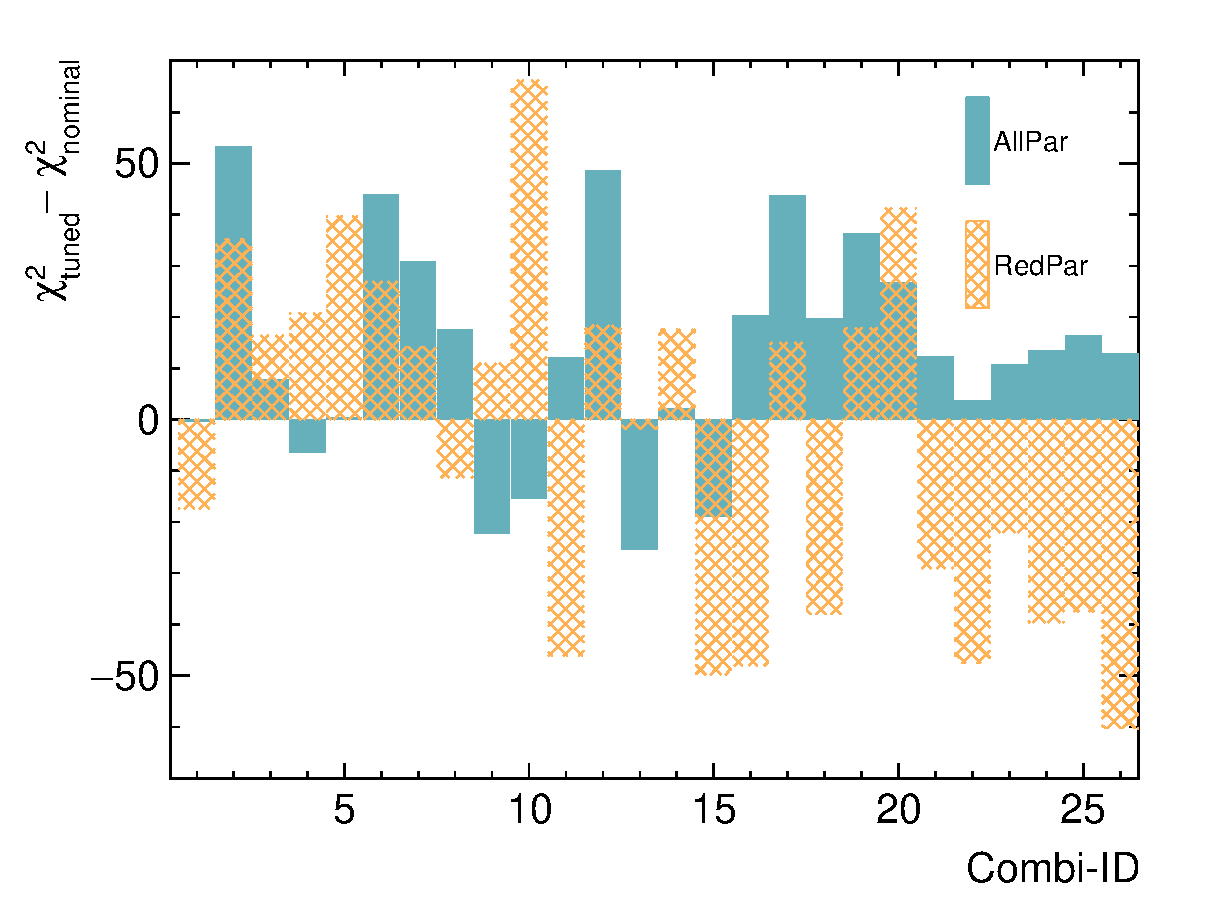
\includegraphics[width=\sgfigwid\textwidth]{figures/tuning/chi2_hist_covfix.eps} 
        \caption{\label{fig:allchi} Change of $\chi^2$ calculated for the full (i.e., tuned plus validation) observable set as a function of the tuned combination (cf. Table~\ref{tab:fit-var-combo}). The two model parameter sets (\allpar and \redpar, see Table~\ref{tab:restunes} for definitions) are compared and it can be seen that the respective minima happen at \texttt{Combi-13} and 26. }   
    \end{figure}
    The largest reduction in $\chi^2$ is -25.39 for \texttt{Combi-13}, denoted as \cbAllPar\ for subsequent discussion.
    The parameters resulted from this tune are referred to as \gT\ for conciseness and are summarized in Table~\ref{tab:restunes}, in which the upper part contains the parameter values and the lower section illustrates $\chi^2$ improvements for selected observables and their corresponding validation sets. 

    MC predictions using \gT\ are compared to the data in Fig.~\ref{fig:g24-t-dat-reac} and Fig.~\ref{fig:g24-t-pn-reac} for the $\dat$ and $\pn$ measurements, respectively.
    \begin{figure*} 
        \centering 		
        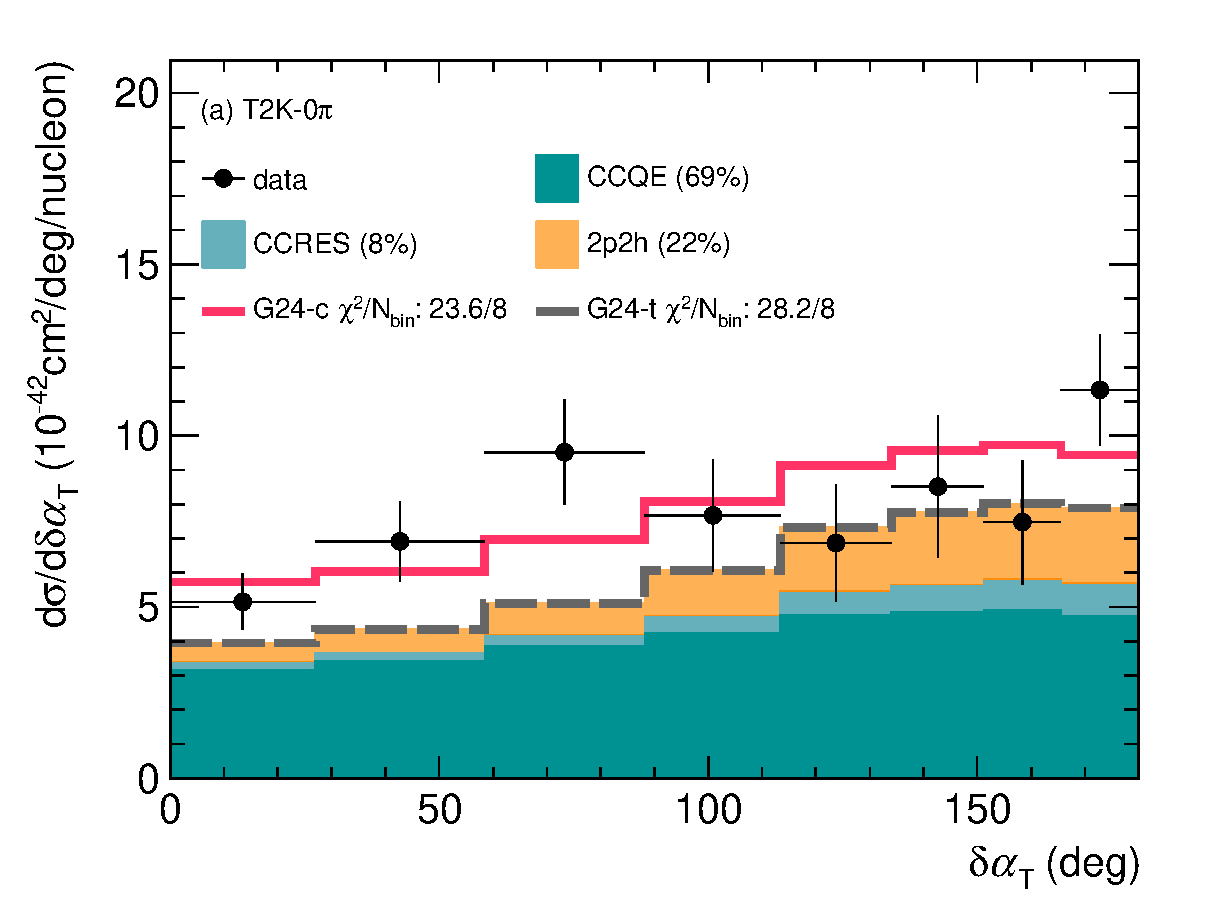
\includegraphics[width=\dbfigwid\textwidth]{figures/tuning/0013-t2k_0pi_dalphat_reac_decomp.eps}
        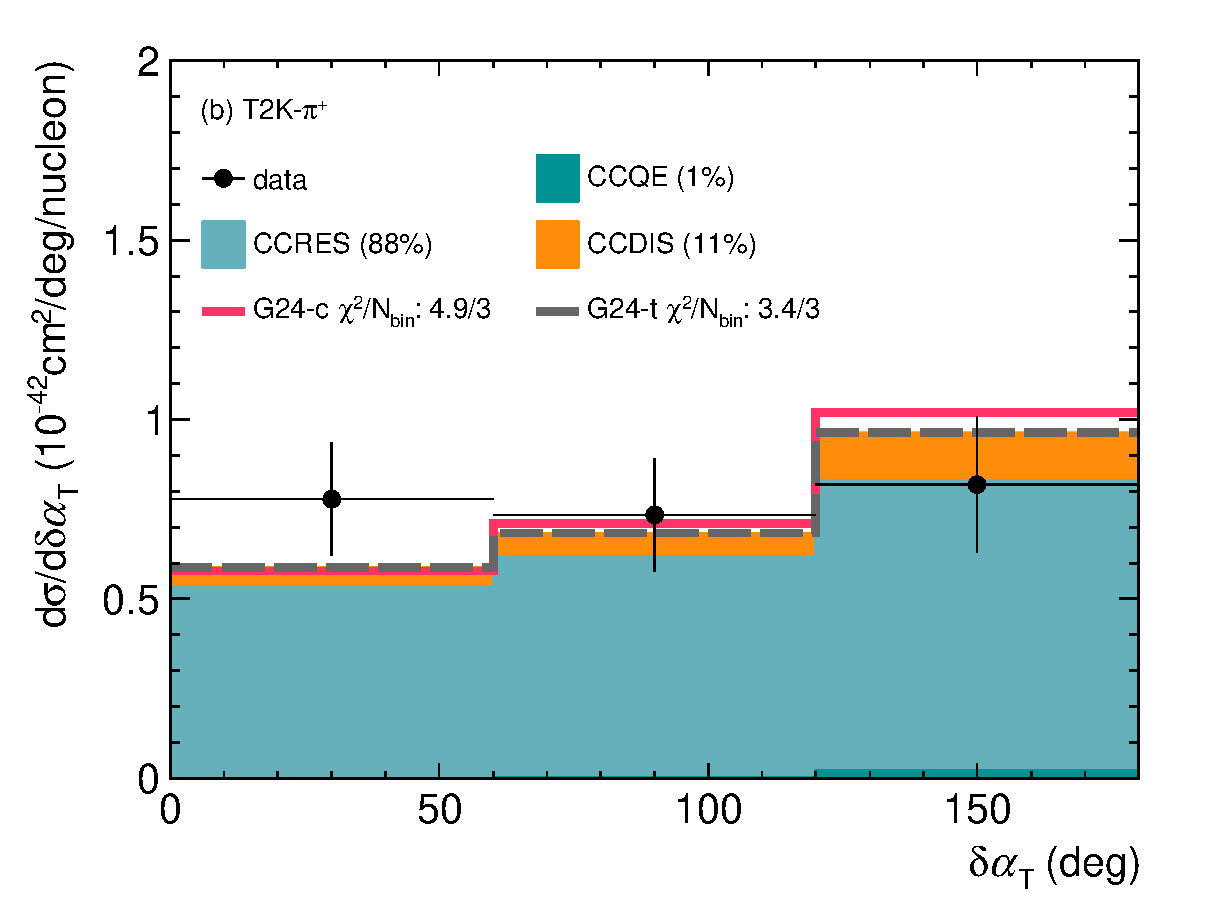
\includegraphics[width=\dbfigwid\textwidth]{figures/tuning/0013-t2k_pip_dalphat_reac_decomp.eps}
        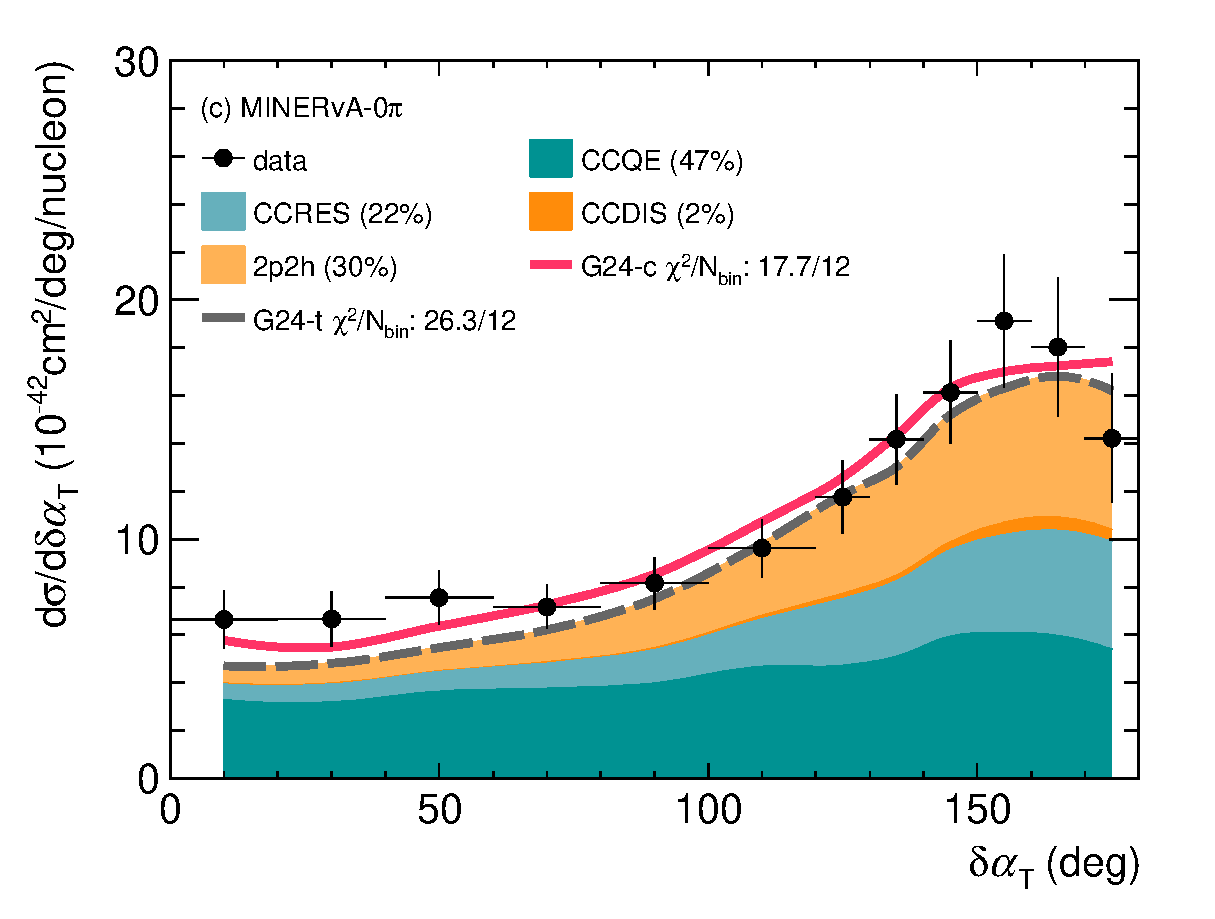
\includegraphics[width=\dbfigwid\textwidth]{figures/tuning/0013-min_0pi_dalphat_reac_decomp.eps}
        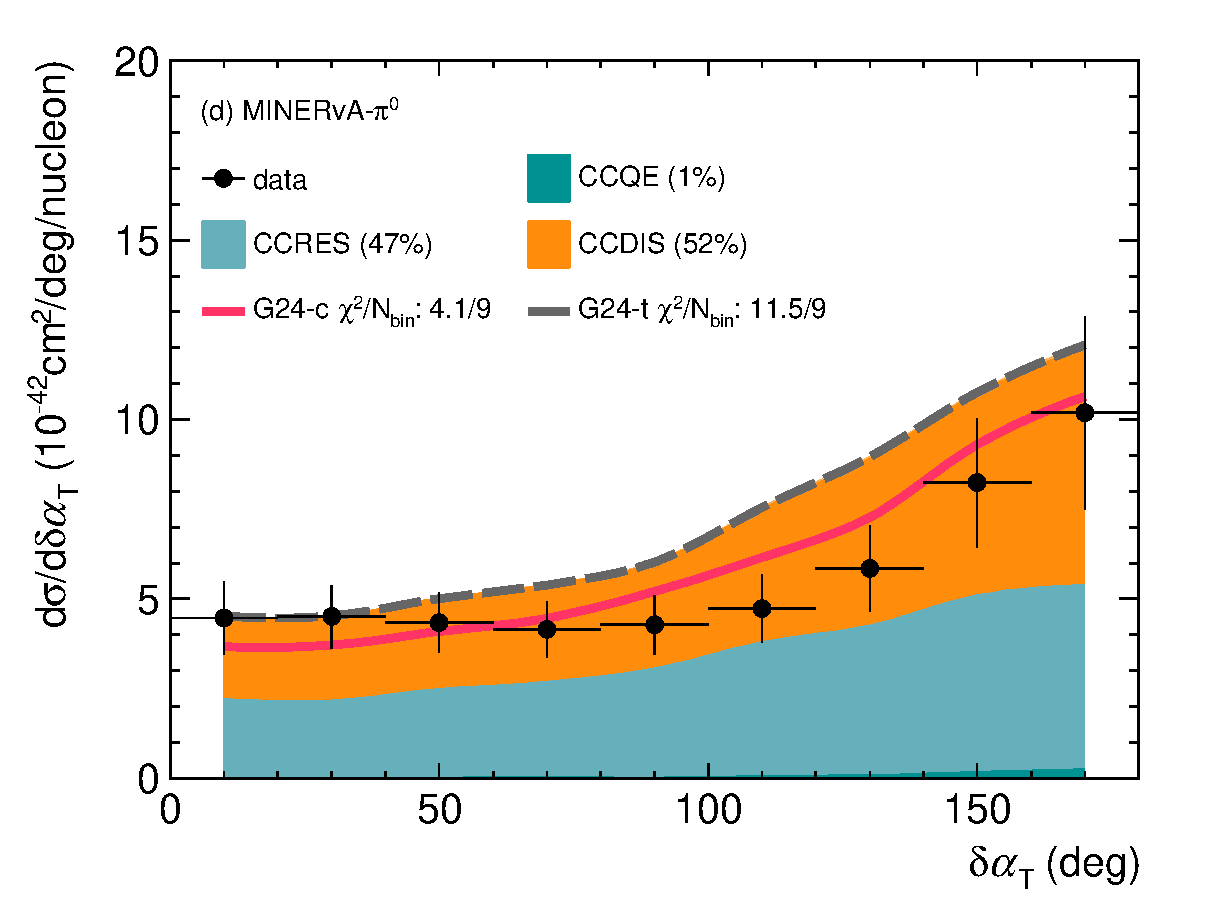
\includegraphics[width=\dbfigwid\textwidth]{figures/tuning/0013-min_pi0_dalphat_reac_decomp.eps}
        \caption{\label{fig:g24-t-dat-reac} 
        Similar to Fig.~\ref{fig:g24-0-dat-reac} but with \gT. The \gC, the best tune obtained (see next subsection), prediction is also plotted for comparison. 
        } 

        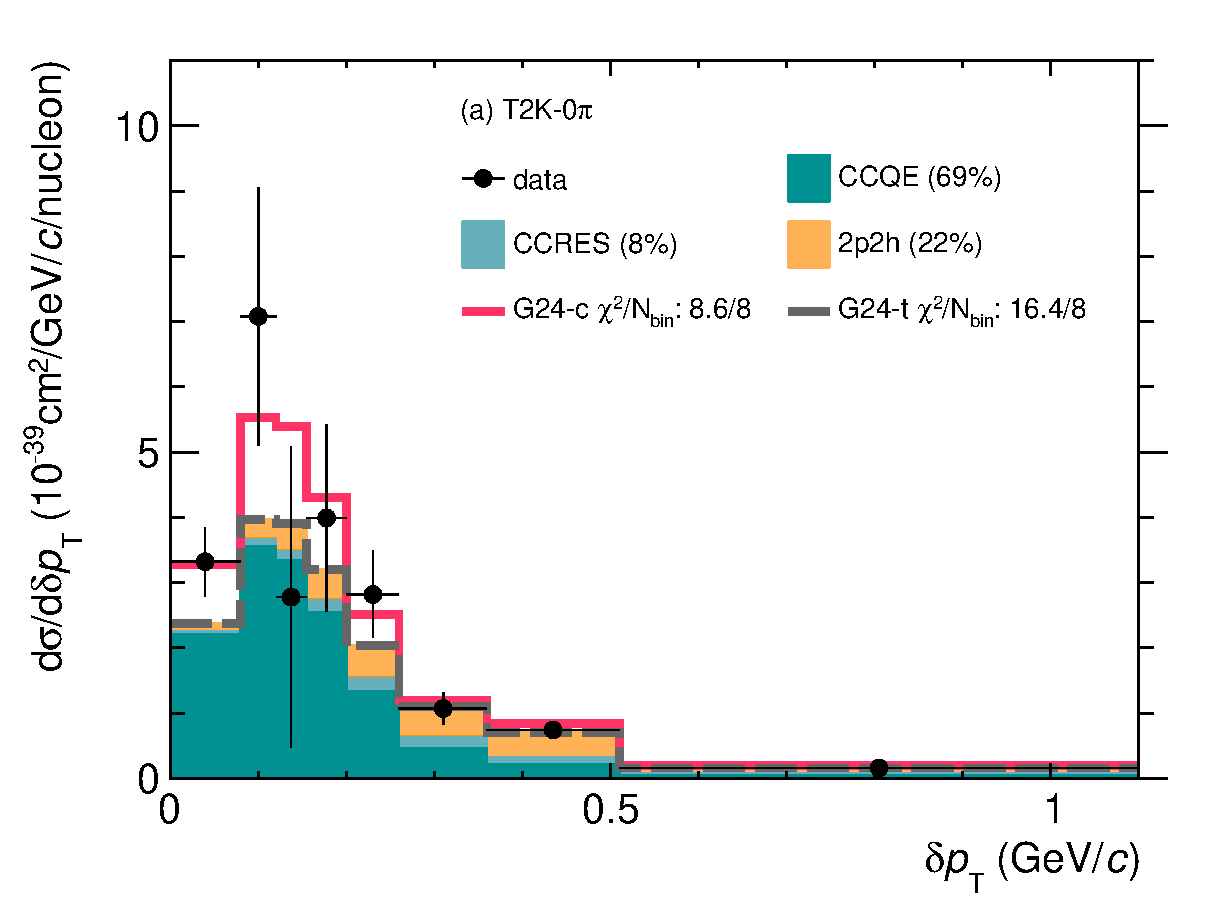
\includegraphics[width=\dbfigwid\textwidth]{figures/tuning/0013-t2k_0pi_dpt_reac_decomp.eps}
        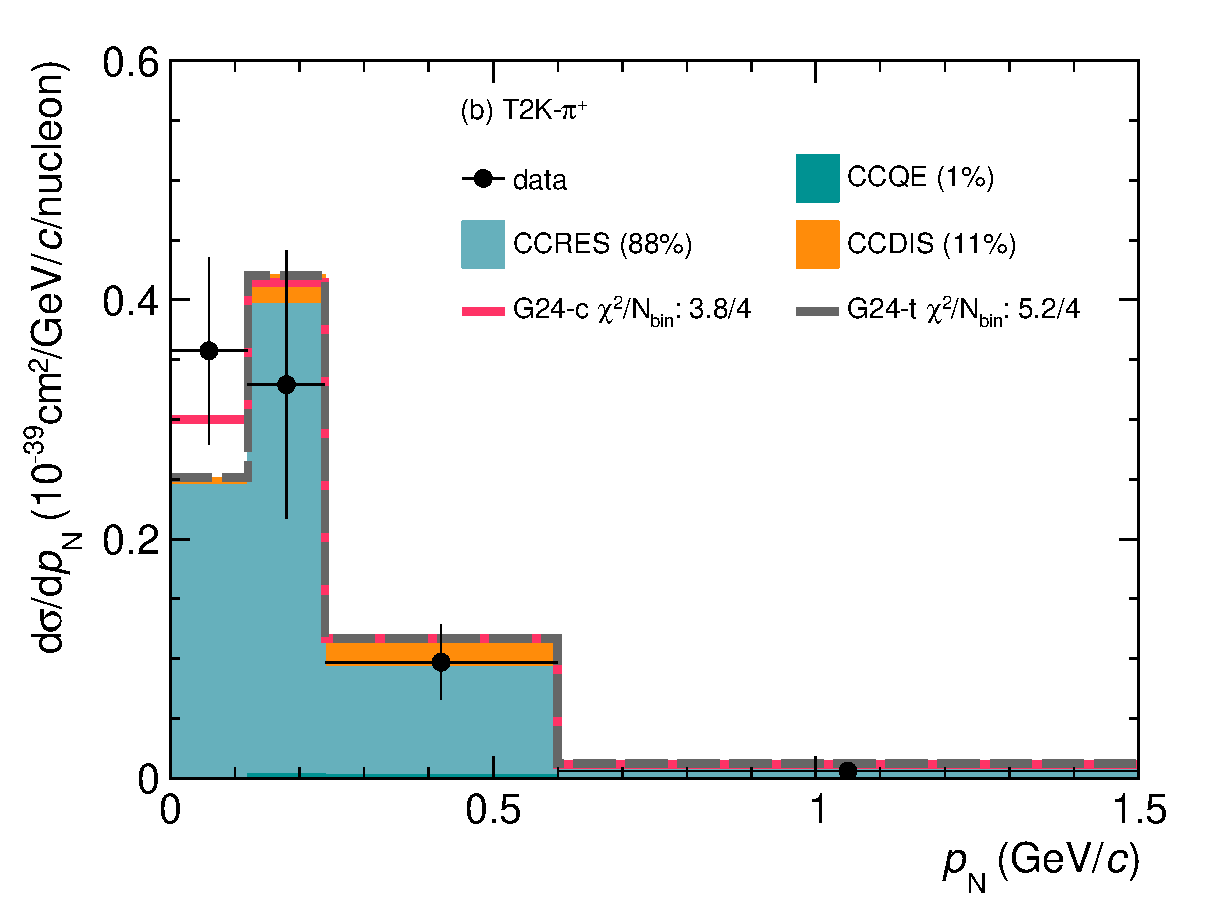
\includegraphics[width=\dbfigwid\textwidth]{figures/tuning/0013-t2k_pip_pn_reac_decomp.eps}	
        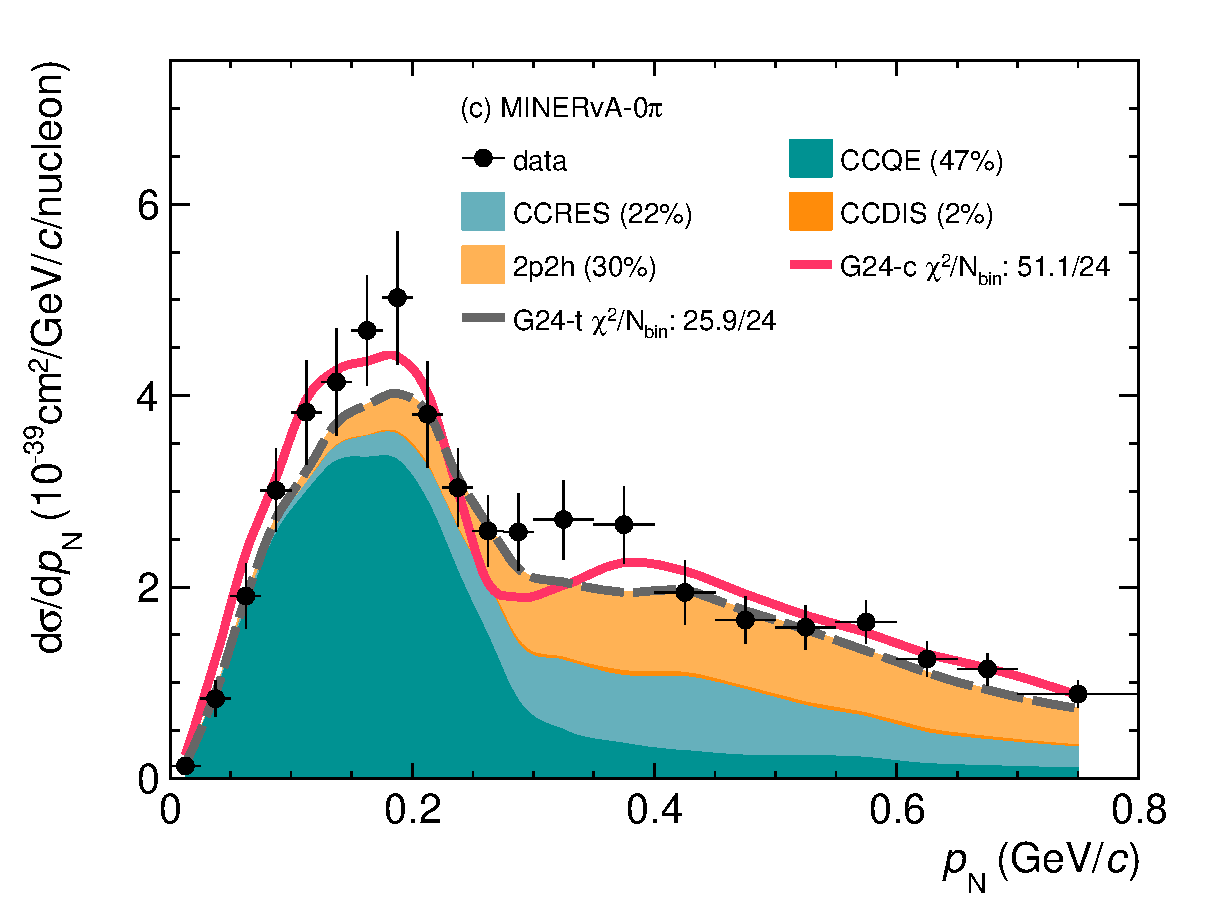
\includegraphics[width=\dbfigwid\textwidth]{figures/tuning/0013-min_0pi_pn_reac_decomp.eps}
        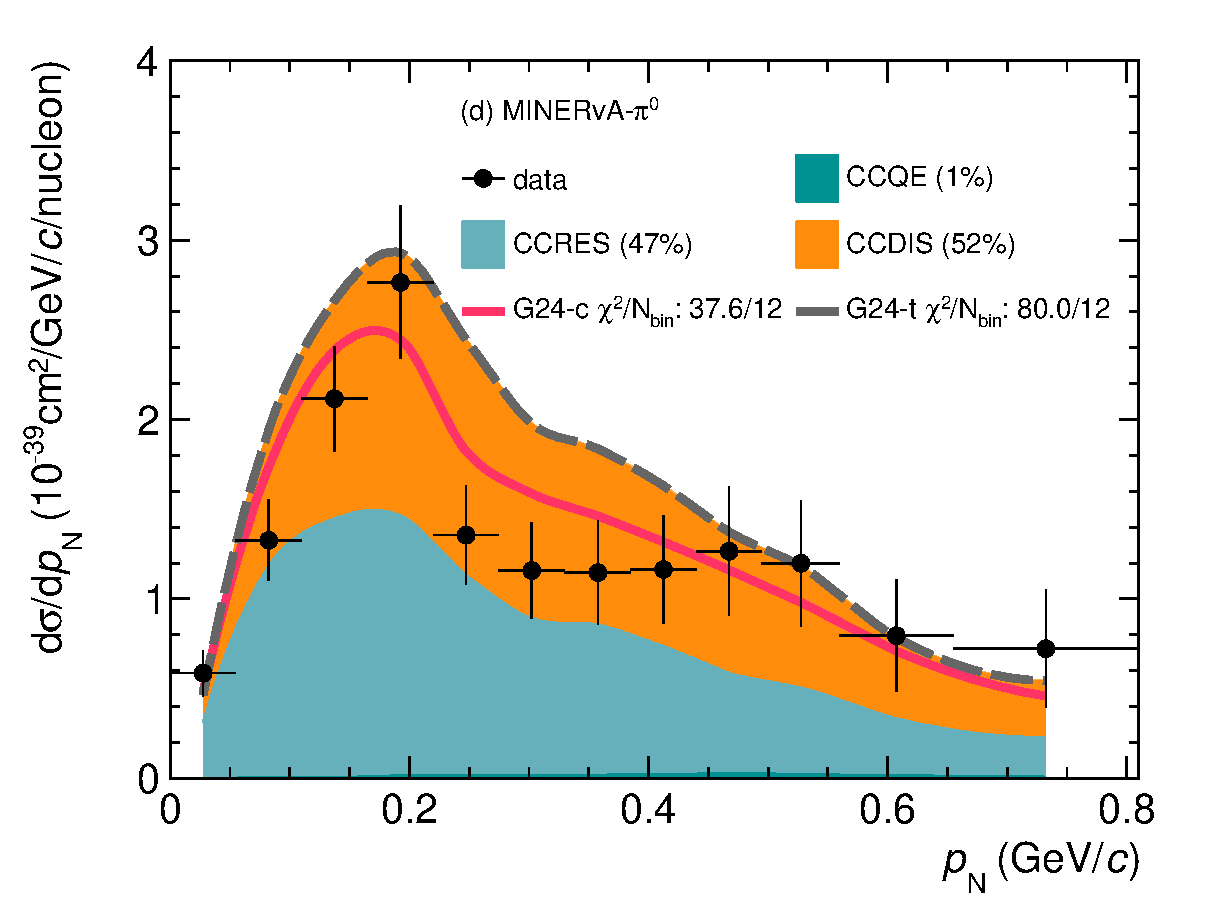
\includegraphics[width=\dbfigwid\textwidth]{figures/tuning/0013-min_pi0_pn_reac_decomp.eps}
        \caption{\label{fig:g24-t-pn-reac}  
        Similar to Fig.~\ref{fig:g24-t-dat-reac} but for the $\pn$ (\ttkpip, \minzpi\ and \minpiz) and $\dpt$ (\ttkzpi) measurements. 
        } 
    \end{figure*}
    It is interesting that the decrease in $\chi^2$ for \gT\ mainly comes from the validation set, as evident in the small $\chi^2$ for $\pn$ of \minzpi\ in Fig.~\ref{fig:g24-t-pn-reac}.

    % To further investigate the improvement, \gT, illustrated in Fig.~\ref{fig:minpiz-alttune}. 
    The most prominent change of \gT\ is the noticeable increase of $\srcfr$ from $0.12$ to $0.17$, while all other FSI fates are close to the nominal values.
    This increases the high energy tail in the $\pn$ distribution, raising the dip in the MC prediction of the $\pn$ distribution between $250~\mevc$ and $300~\mevc$ and moving the distribution peak to the appropriate place, thereby closing the gap between the data and the MC prediction in the high energy region.
    However, as the \minpiz\ $\pn$ prediction using \gZero\ is already higher than data, this increase in $\srcfr$ does not improve the data-MC agreement for \minpiz.
    Overall, this leads to a moderate reduction of $25.39$ in $\chi^2$ (Table~\ref{tab:restunes}), as well as a relatively improved data-MC agreement across all data sets. 
    % \begin{figure}[!htb] 	
    %     \centering 		
    %     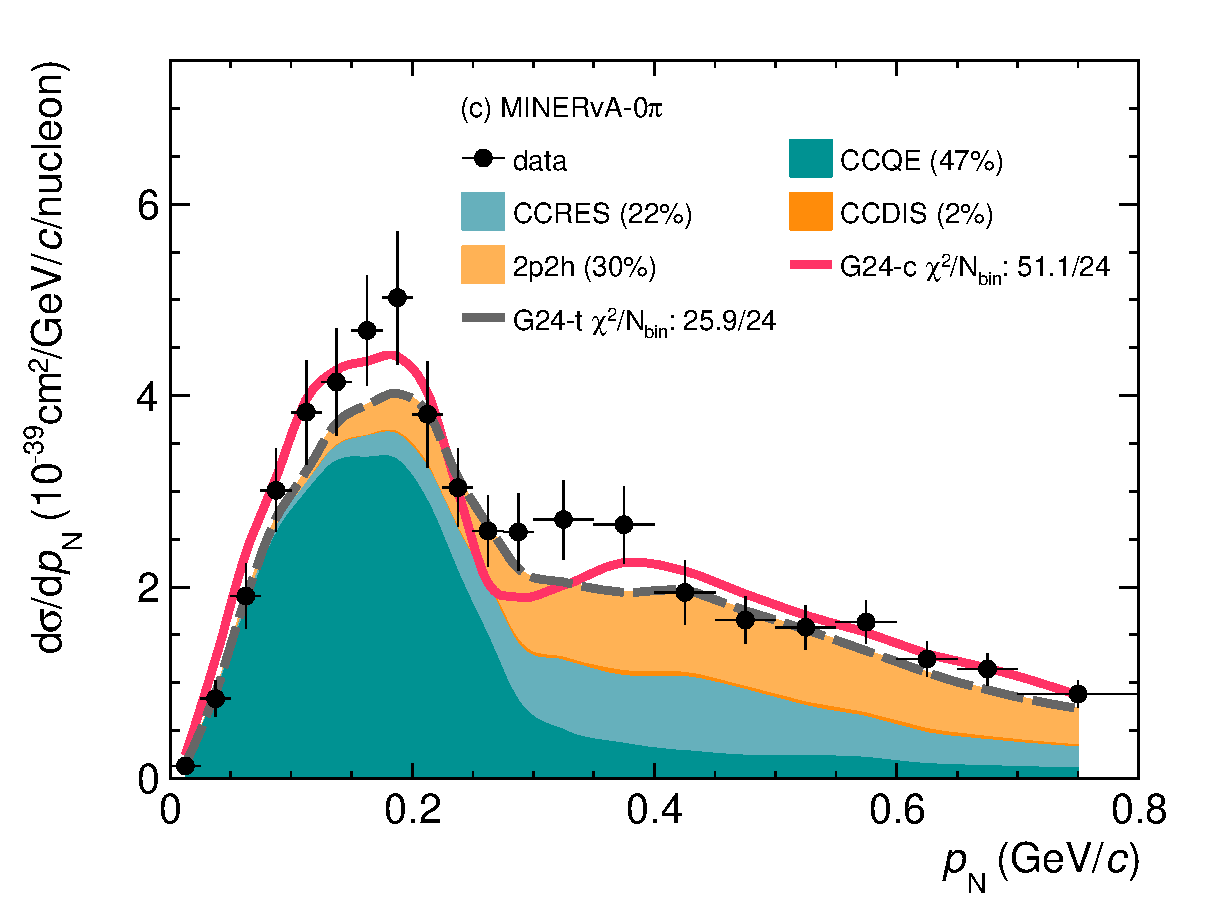
\includegraphics[width=\trfigwid\textwidth]{figures/tuning/0013-min_0pi_pn_reac_decomp.eps}
    %     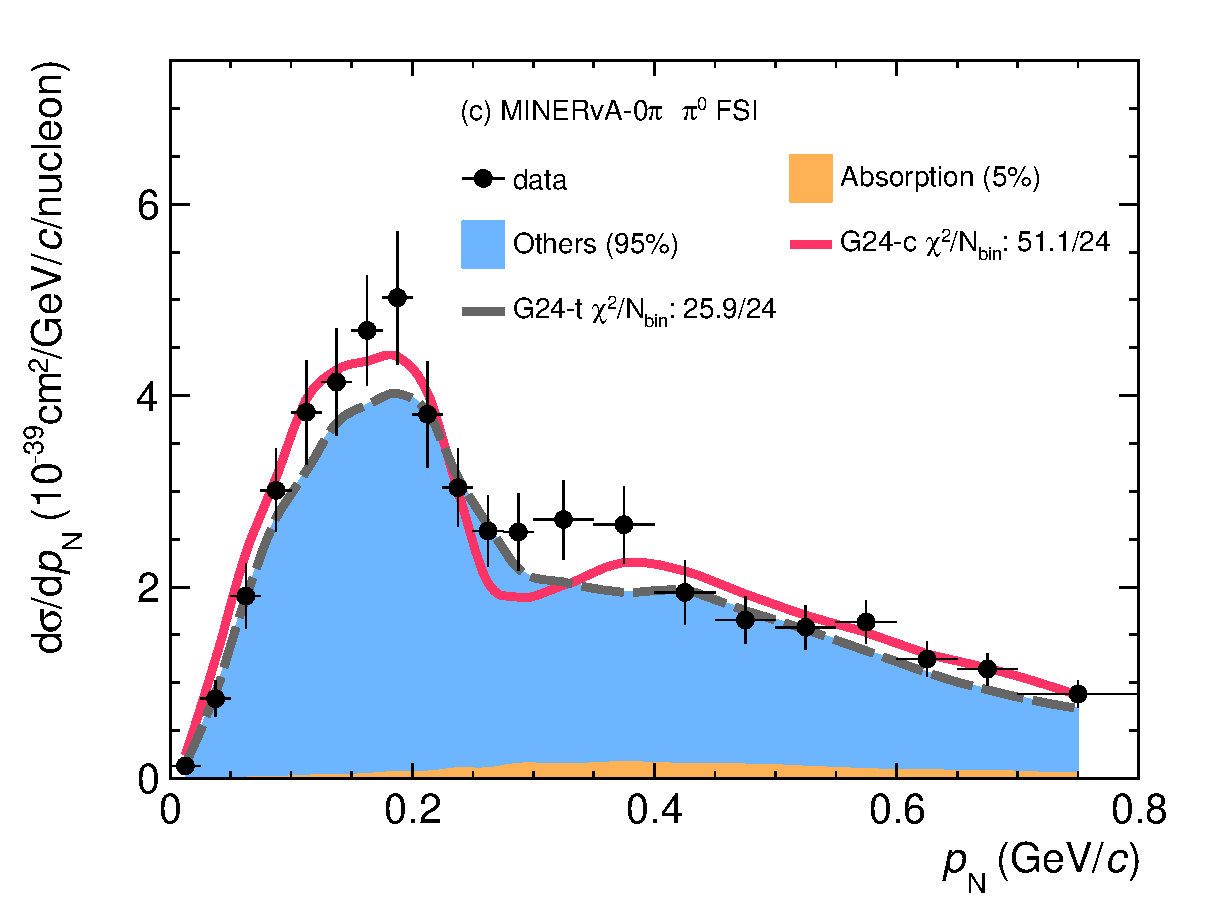
\includegraphics[width=\trfigwid\textwidth]{figures/tuning/0013-min_0pi_pn_pi0_decomp.eps}
    %     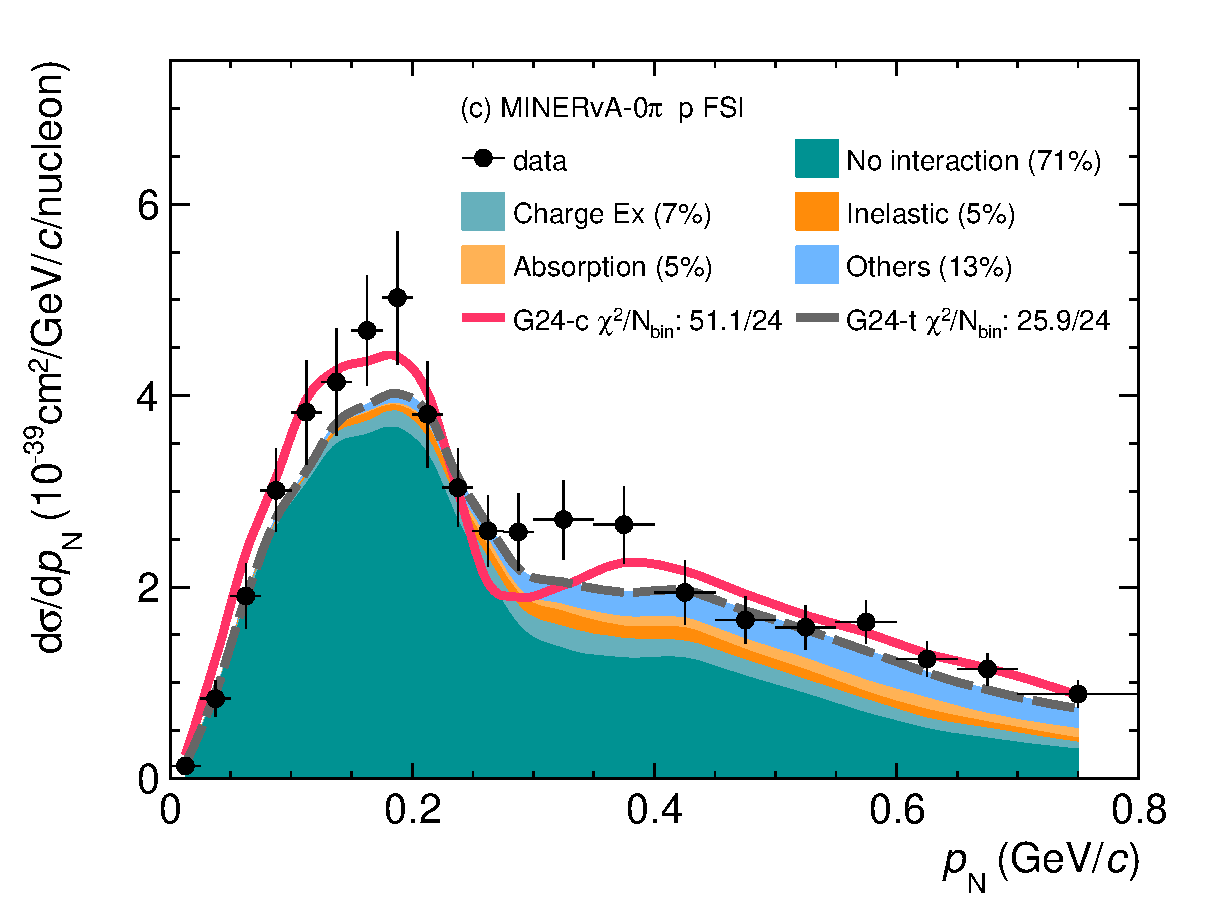
\includegraphics[width=\trfigwid\textwidth]{figures/tuning/0013-min_0pi_pn_pr_decomp.eps}
    %     \caption{\label{fig:minzpi-alttune} \minzpi\ $\pn$ measurement compared to \genie\ predictions decomposed in  (a) $\nu$-N interaction, (b) $\piz$ FSI, and (c) proton FSI for the alternative tune, \gT.} 
    % \end{figure}
    Regarding the other combinations of data sets, there does not seem to be a consistent pattern regarding to observable combinations with respect to the $\chi^2$ reduction.
    For example, as \minpiz\ has the largest deviation, one might expect that the combinations containing \minpiz\ would have larger reduction in $\chi^2$. 
    This is true for \texttt{Combi-13}, which includes only the pion data, i.e. \ttkpip\ and \minpiz, but not for \texttt{Combi-11}, which includes only MINERvA data, i.e. \minzpi\ and \minpiz.
    Unexpectedly, the majority of the combinations yield an increase in $\chi^2$.
    This could be due to the intricate correlations among model parameters, so correlation between \allpar\ in the tuning using \cbAllPar\ is plotted in Fig.~\ref{fig:comb_26_cor_allpar}.
    Indeed, considerable correlation and anti-correlation are observed between different FSI fates for the same particle, e.g. $\cpiabs$ and $\pipiprod$. 
    \begin{figure}[!htb] 	
        \centering 		
        \begin{subfigure}{\dbfigwid\textwidth}
            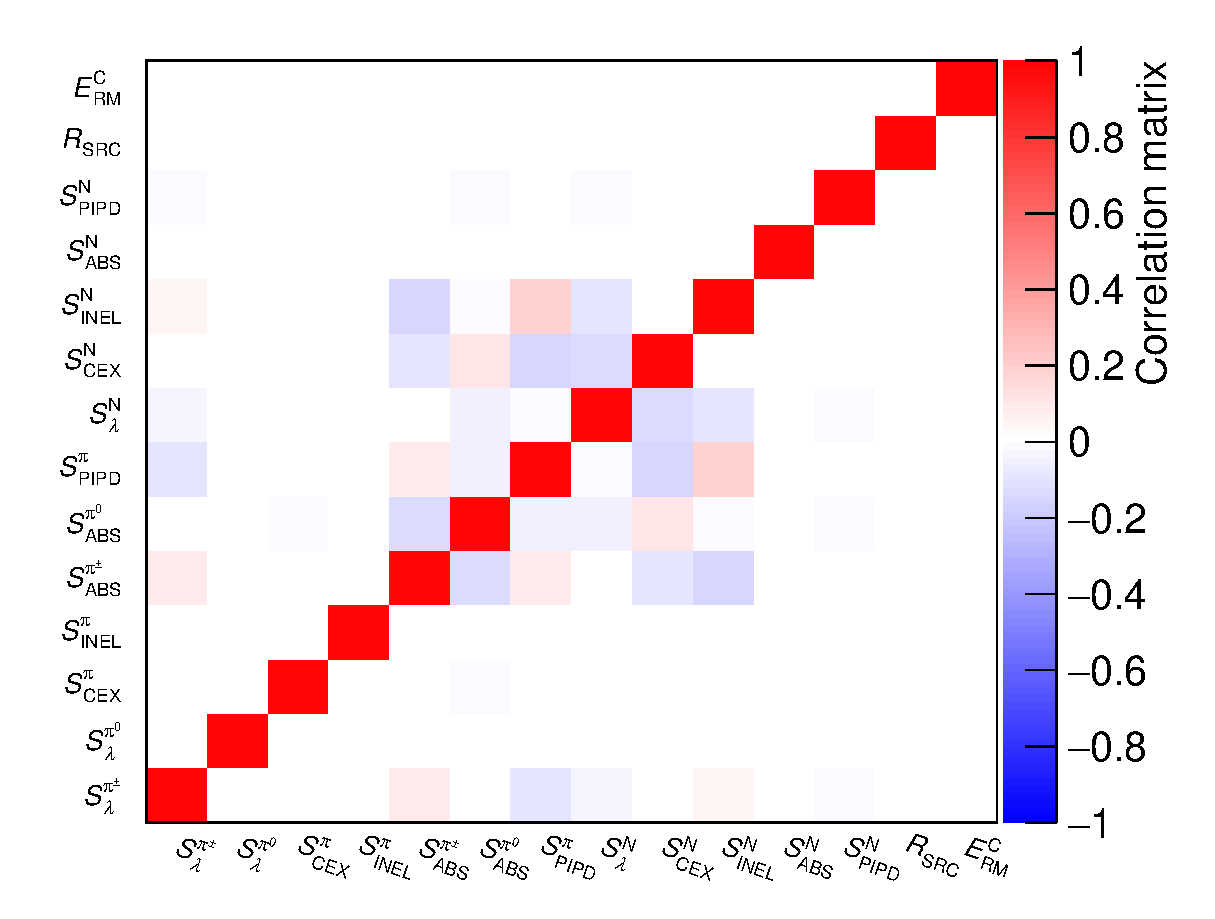
\includegraphics[width=\textwidth]{figures/tuning/result_test_comb_26_cor_allpar_covfix.eps}
            \caption{\allpar}
            \label{fig:comb_26_cor_allpar}
        \end{subfigure}
        \begin{subfigure}{\dbfigwid\textwidth}
            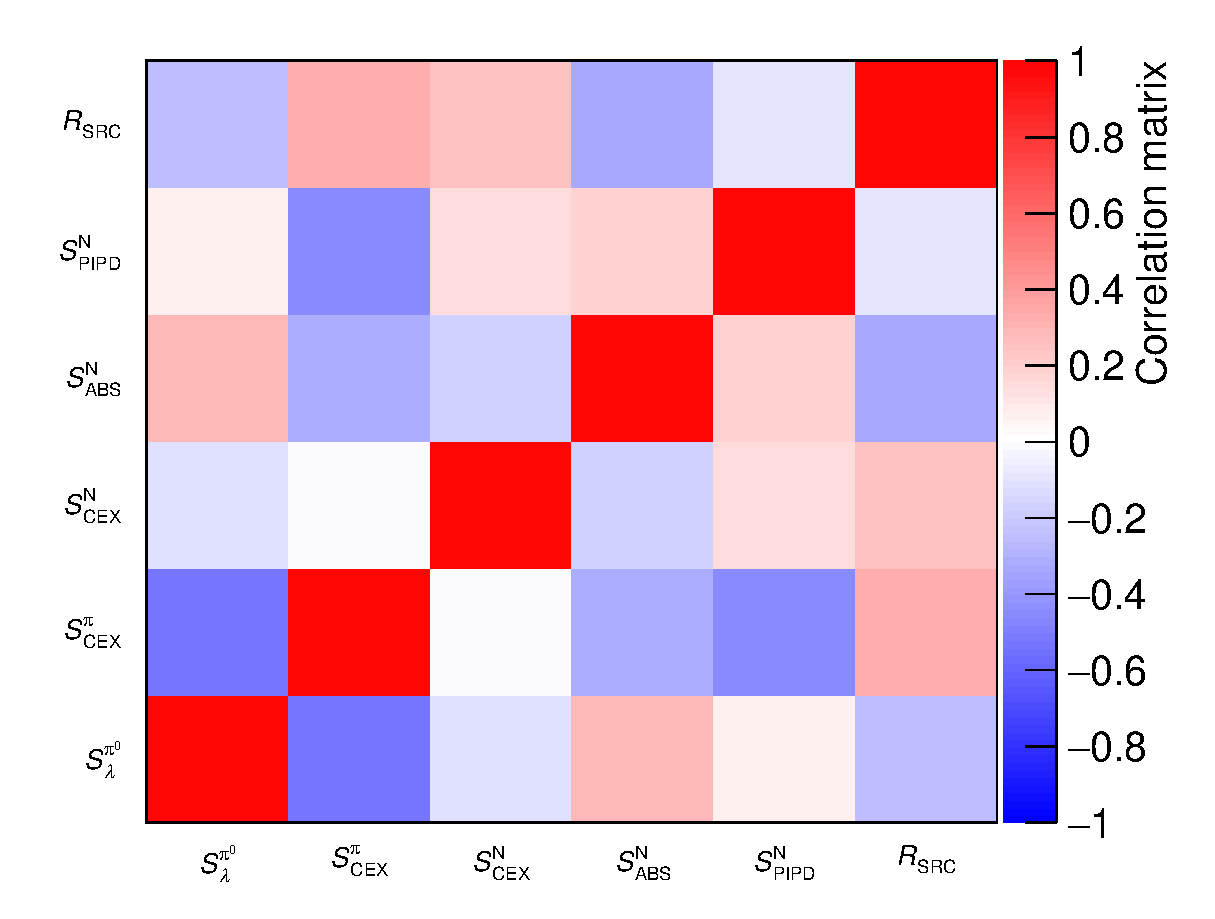
\includegraphics[width=\textwidth]{figures/tuning/result_test_comb_26_cor_redpar_covfix.eps}
            \caption{\redpar}
            \label{fig:comb_26_cor_redpar}
        \end{subfigure}
        \caption{ Post-fit Correlation coefficient on \texttt{Combi-26}. } 
    \end{figure}

    Moreover, it was observed that for most combinations, several parameters stayed near their nominal values—typically within one standard deviation of the imposed priors. 
    For instance, $\pipiprod$ remained largely unchanged since no data set significantly constrains the PIPD contribution of pions, indicating that excluding these parameters from the tuning has little effect on the results.
    Consequently, we constructed a reduced set consisting only of $\srcfr$, $\pizmfp$, $\picex$, $\ncex$, $\nabs$, and $\npiprod$ (denoted as \redpar\ in Table~\ref{tab:restunes}) and applied the tuning procedure to all 26 observable combinations using this parameter subset.
    Note that only one of the set of considerably correlated parameters, shown by the central square in Fig.~\ref{fig:comb_26_cor_allpar}, namely $\ncex$ is present in \redpar. 


    \subsection{\redpar\ tune}
    The \redpar\ tuning proved more stable, with the majority of combinations showing a more negative $\chi^2$ change than the \allpar\ tuning, as shown in Fig.~\ref{fig:allchi}. 
    The most significant reduction in $\chi^2$ is observed for \texttt{Combi-26} (referred to as \cbRedPar\ in Table~\ref{tab:fit-var-combo}). 
    This combination selects all TKI observables except for $\dphit$ and $\dpt$—namely, $\dat$, $\pn$ (or $\dpt$ if $\pn$ is missing), and $\dptt$—from both pionless and pion-production measurements in T2K and MINERvA.

    The $\chi^2$ improvement for \cbRedPar\ is -60.28, which is significantly better than the improvement obtained with \cbAllPar\ tuning.
    The parameters obtained from this tuning are referred to as \gC\ for conciseness and are summarized in Table~\ref{tab:restunes}.
    The main reduction in $\chi^2$ for \gC\ comes from the tuned observables, which is as expected, and it is also encouraging that the validation observables have a negligible change of $2.8$ in $\chi^2$.
    The MC predictions using \gC\ are compared to the data in Fig.~\ref{fig:g24-c-dat-reac} and Fig.~\ref{fig:g24-c-pn-reac} for the $\dat$ and $\pn$ measurements, respectively.
    \begin{figure*} 
        \centering 		
        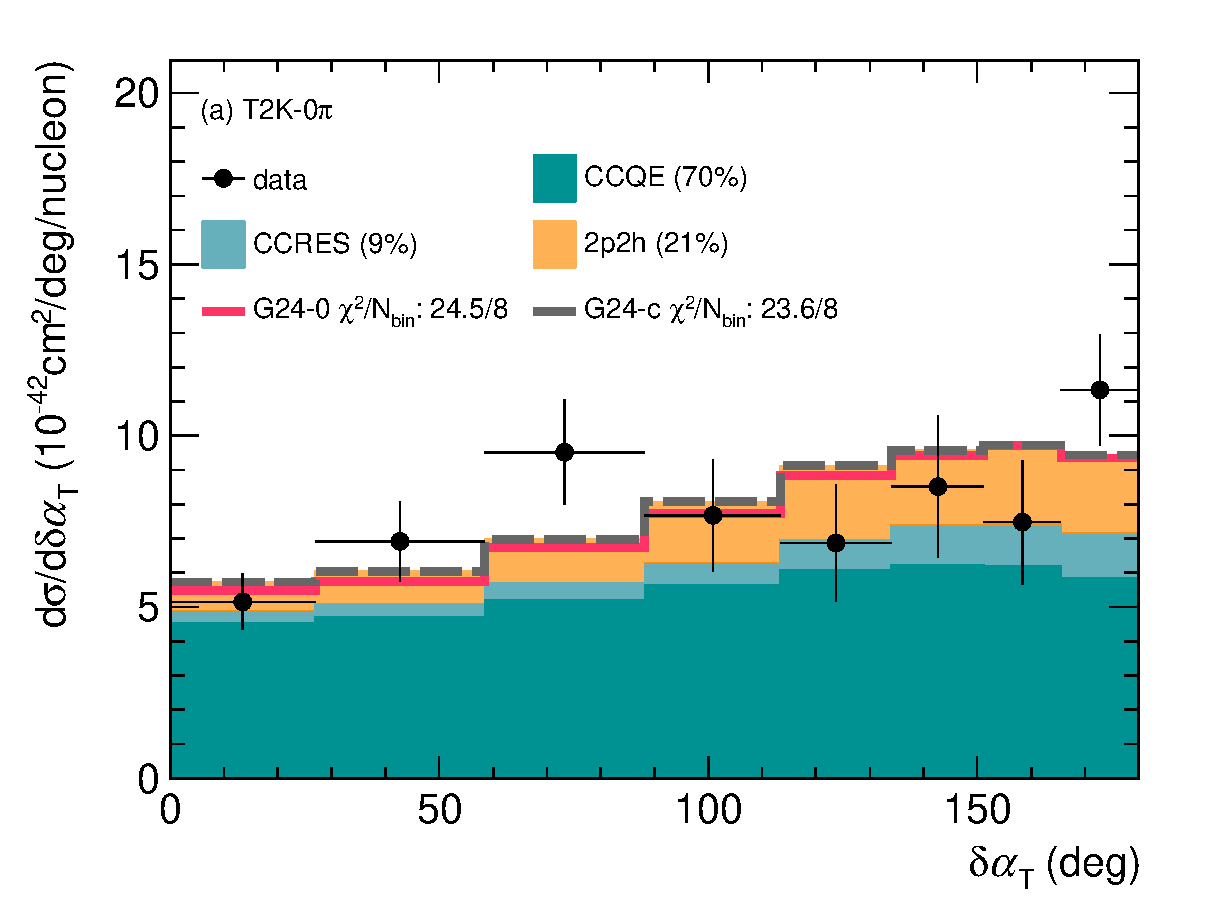
\includegraphics[width=\dbfigwid\textwidth]{figures/tuning/0026-t2k_0pi_dalphat_reac_decomp_covfix.eps}
        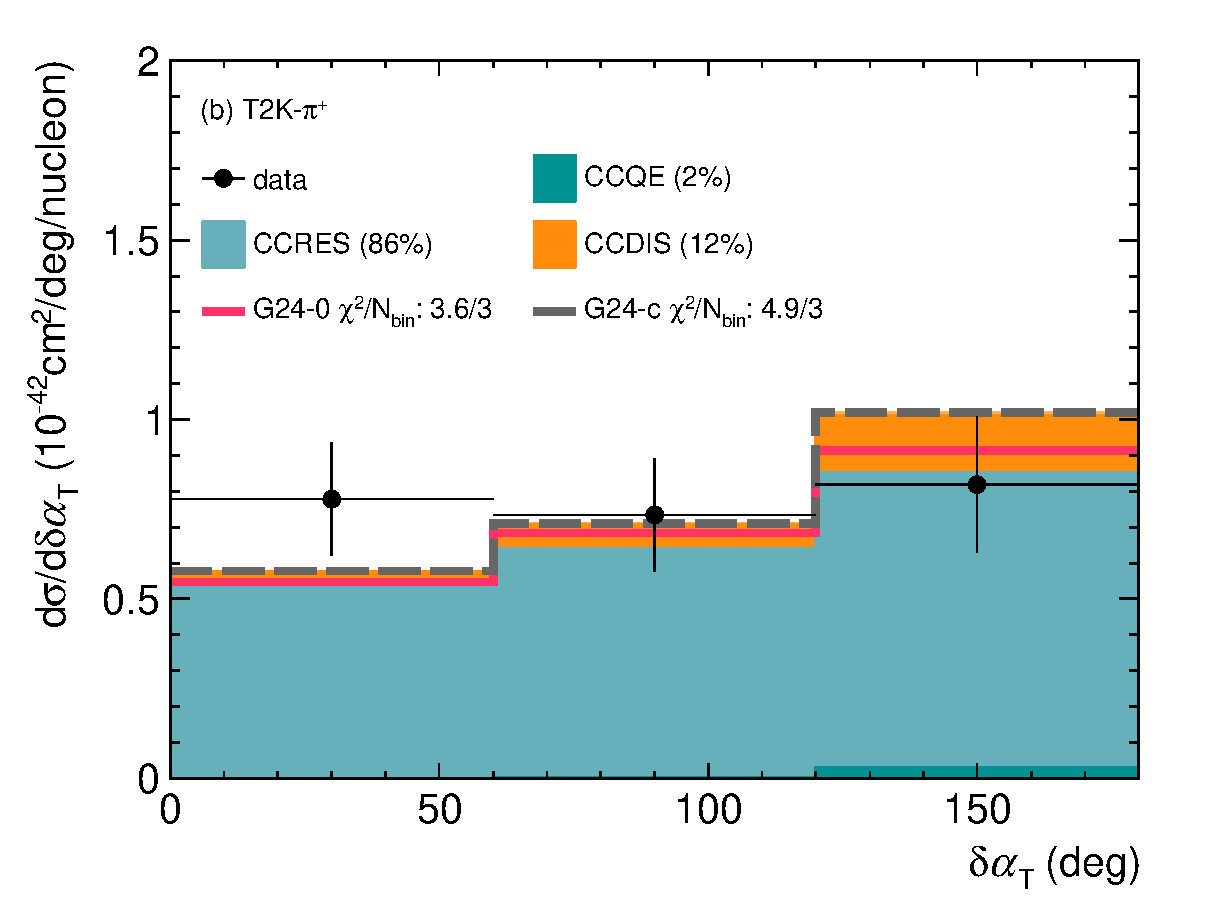
\includegraphics[width=\dbfigwid\textwidth]{figures/tuning/0026-t2k_pip_dalphat_reac_decomp_covfix.eps}
        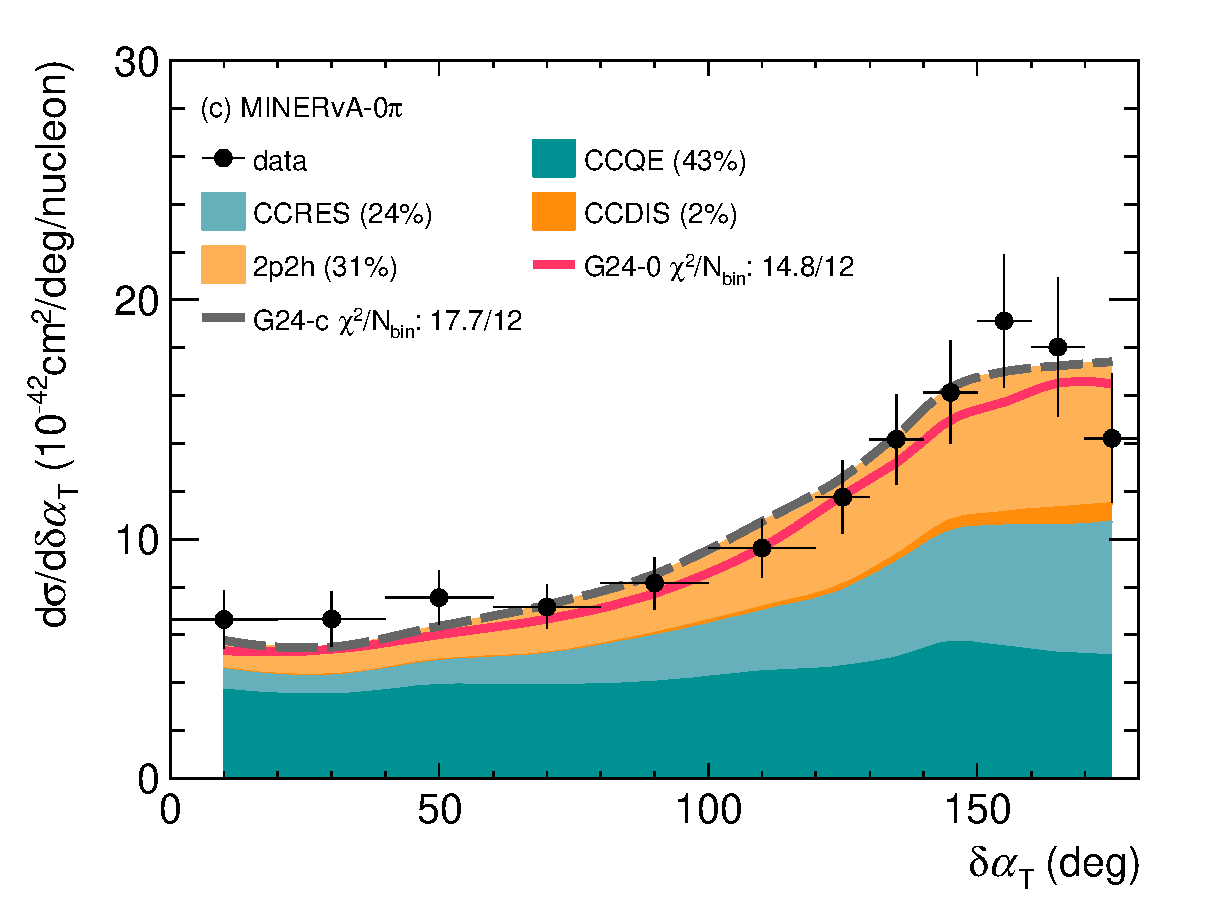
\includegraphics[width=\dbfigwid\textwidth]{figures/tuning/0026-min_0pi_dalphat_reac_decomp_covfix.eps}
        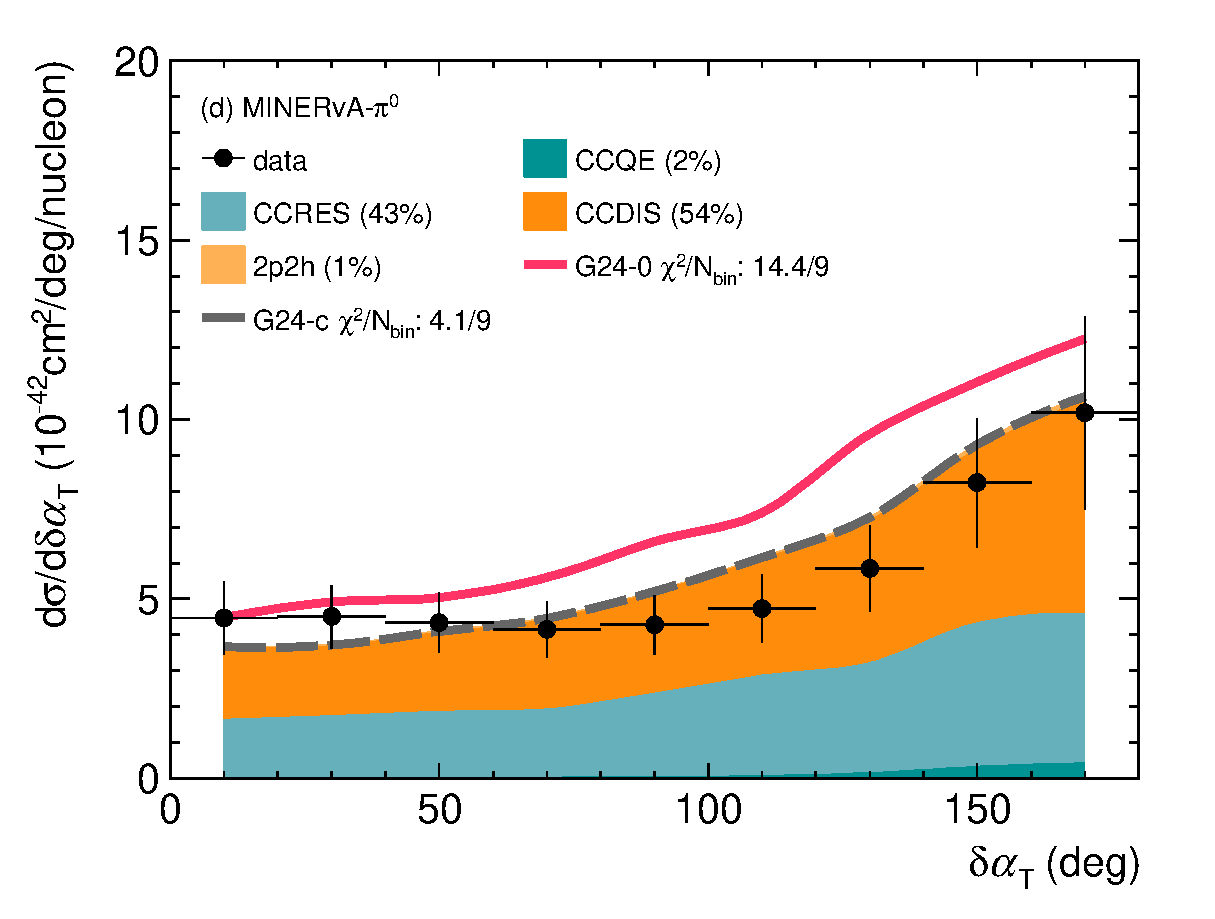
\includegraphics[width=\dbfigwid\textwidth]{figures/tuning/0026-min_pi0_dalphat_reac_decomp_covfix.eps}
        \caption{\label{fig:g24-c-dat-reac} 
        Similar to Fig.~\ref{fig:g24-0-dat-reac} but with \gC.  The \gZero\ prediction is also plotted for comparison. 
        } 

        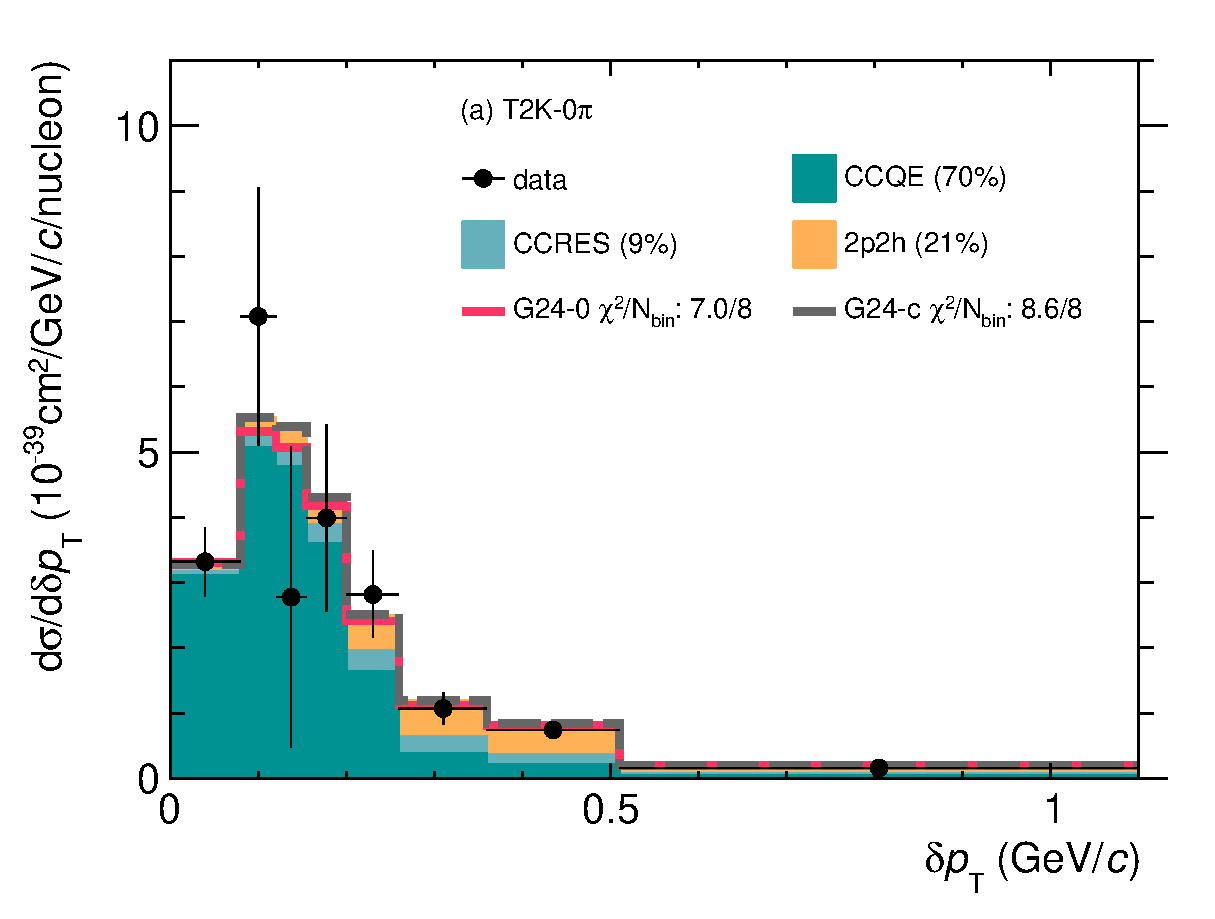
\includegraphics[width=\dbfigwid\textwidth]{figures/tuning/0026-t2k_0pi_dpt_reac_decomp_covfix.eps}
        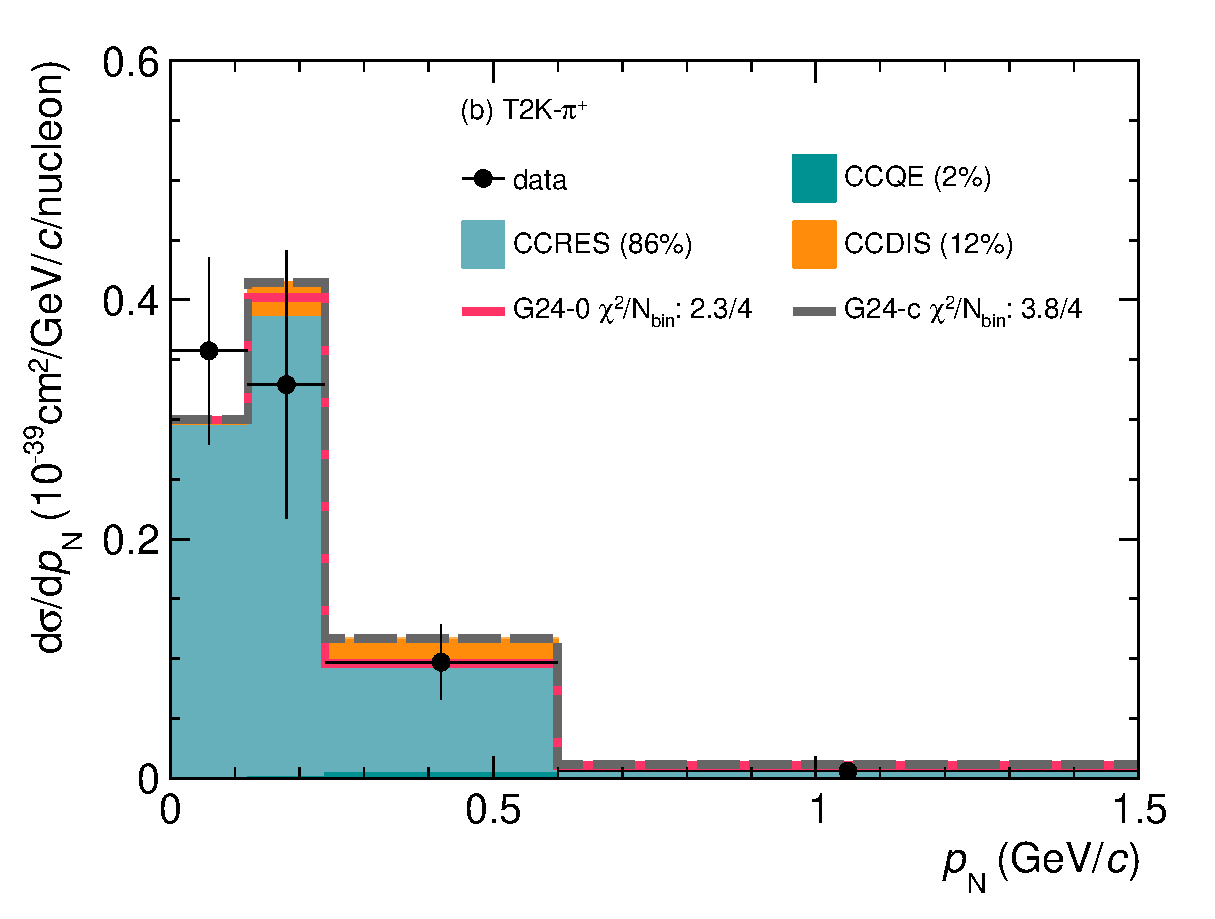
\includegraphics[width=\dbfigwid\textwidth]{figures/tuning/0026-t2k_pip_pn_reac_decomp_covfix.eps}	
        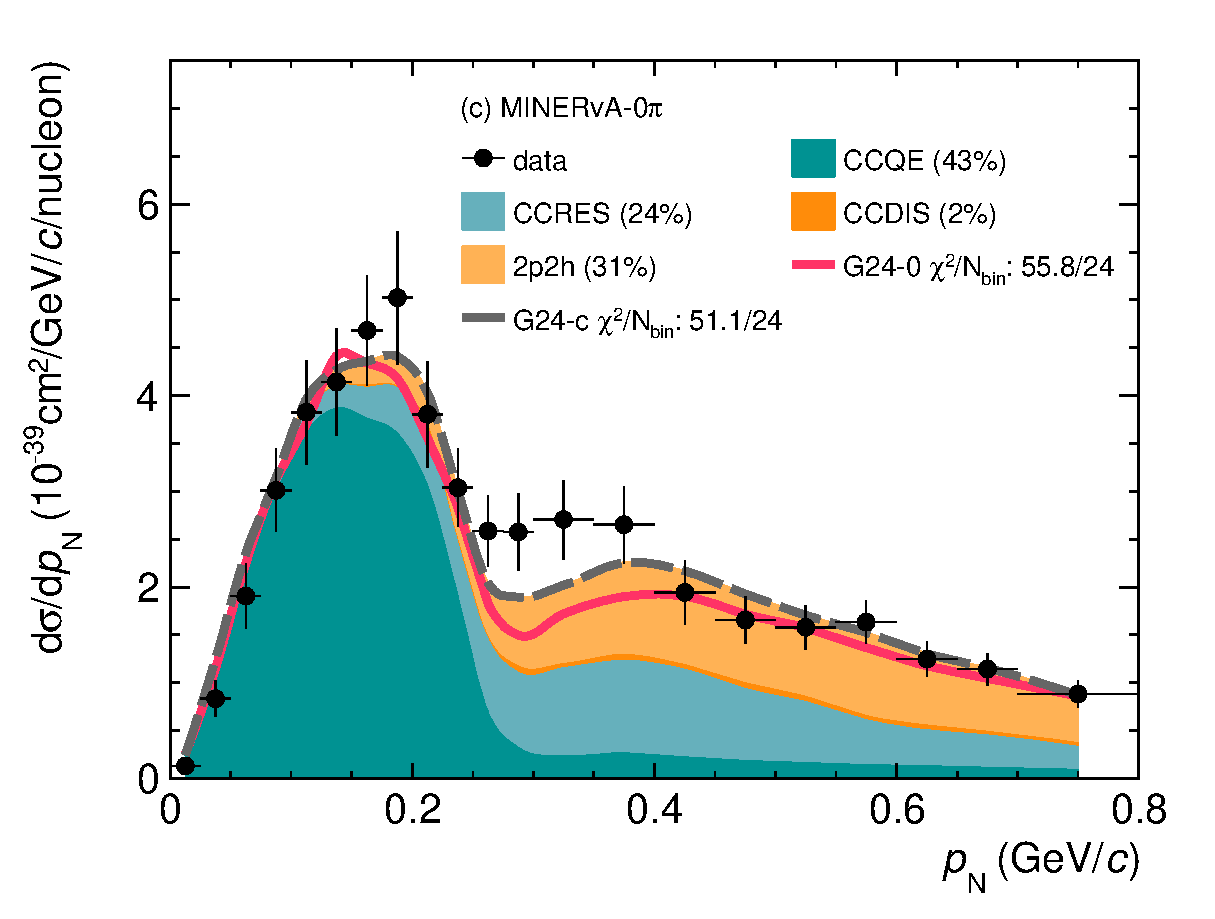
\includegraphics[width=\dbfigwid\textwidth]{figures/tuning/0026-min_0pi_pn_reac_decomp_covfix.eps}
        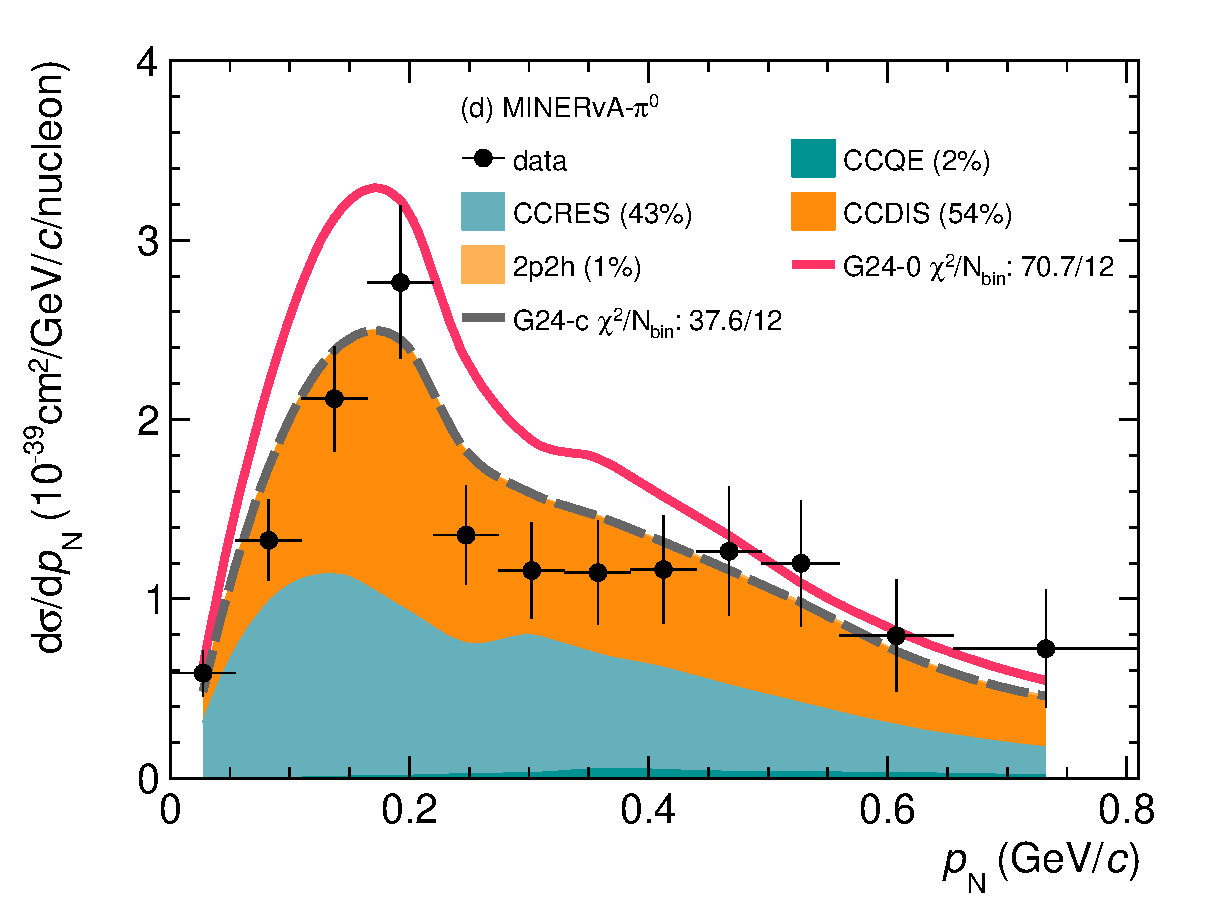
\includegraphics[width=\dbfigwid\textwidth]{figures/tuning/0026-min_pi0_pn_reac_decomp_covfix.eps}
        \caption{\label{fig:g24-c-pn-reac}  
        Similar to Fig.~\ref{fig:g24-c-dat-reac} but for the $\pn$ (\ttkpip, \minzpi\ and \minpiz) and $\dpt$ (\ttkzpi) measurements. 
        } 
    \end{figure*}

    For the \gC\ tune, the modifications to the \sfcfg\ model are moderate (with $\srcfr$ decreasing from $0.12$ to $0.09$), whereas in the hA model both $\pizmfp$ and $\picex$ are substantially suppressed, resulting in a nucleon FSI with increased CEX and PIPD and reduced ABS.  
    For the \ttkzpi, \ttkpip, and \minzpi\ datasets, the new $\chi^2$ values remain comparable to those obtained with \gZero, with variations smaller than the degree of freedom. 
    In the case of \minpiz, \gC\ clearly outperforms \gZero, demonstrating that an accurate simultaneous description of both pionless and pion production samples is achievable using constrained parameters from cross-topology TKI tuning. 
    It should be noted that in the region of $\pn\sim0.3~\gevc$, the model deficit previously reported in Ref.~\cite{MINERvA:2018hba} (and shown in Fig.~\ref{fig:g24-0-pn-reac}c) persists even after the fit. 
    This deficit may be attributed to the strength of the 2p2h contribution~\cite{MINERvA:2018hba}, although its exact origin remains a subject of considerable discussion within the community.

    A detailed examination of individual datasets sheds light on the source of the improvement. 
    Figure~\ref{fig:CEX-minpiz-dat-pi0} presents the decomposition of the $\dat$ cross section according to the FSI fates of the $\piz$. 
    In the hA model, primary interaction products undergo only a single rescattering—recorded using a specific rescattering code—and the resulting final-state particles are stored as daughters of the primary products. 
    Thus, the FSI fate responsible for the final particles can be determined by inspecting the rescattering code of their first parent. 
    More specifically, we loop through all final-state particles to identify the leading $\piz$ and examine the rescattering code of its initial parent. 
    \begin{figure}[!htb] 	
        \centering 		
        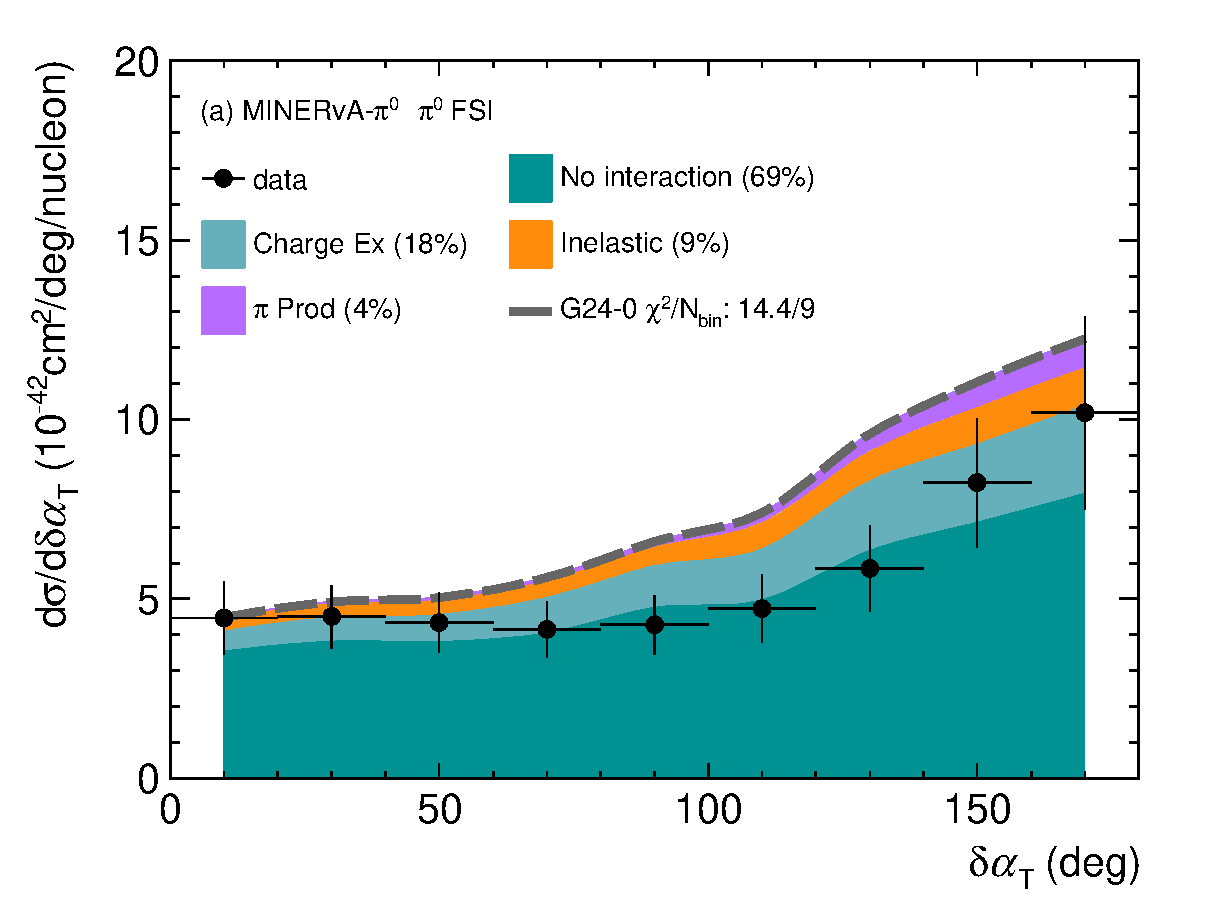
\includegraphics[width=\dbfigwid\textwidth]{figures/tuning/0000-min_pi0_dalphat_pi0_decomp_cex.eps}
        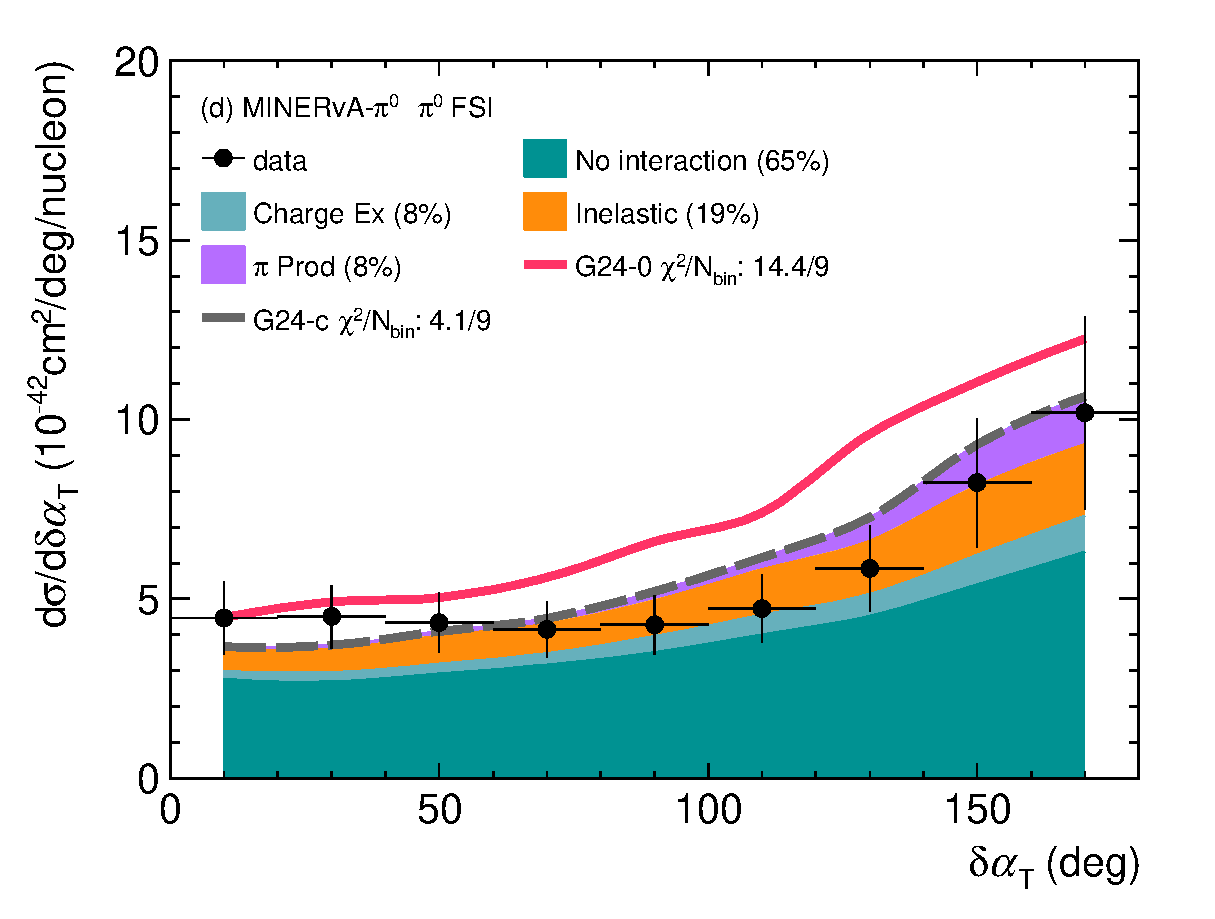
\includegraphics[width=\dbfigwid\textwidth]{figures/tuning/0026-min_pi0_dalphat_pi0_decomp_covfix.eps}	
        \caption{\label{fig:CEX-minpiz-dat-pi0} \minpiz\ $\dat$ measurement compared to \genie\ predictions decomposed in $\piz$ FSI fates with (a) \gZero\ and (b) \gC.} 
    \end{figure}

    In \minpiz, the number of $\piz$s that experience no FSI (``No Interaction'', as shown in the figures) is controlled by the $\pizmfp$ parameter. 
    Reducing $\pizmfp$ diminishes the fraction of ``No Interaction'' events, as illustrated by the comparison between Fig.~\ref{fig:CEX-minpiz-dat-pi0}b and Fig.~\ref{fig:CEX-minpiz-dat-pi0}a. 
    In contrast, an enhancement in $\piz$ rescattering appears in pionless measurements only via ABS. 
    Although there is an increase in ABS for $\piz$ in \ttkzpi\ and \minzpi, the overall fraction is low, resulting in a limited impact. 
    While the increased $\piz$ rescattering could boost \ttkpip\ through CEX (as discussed subsequently), the substantial suppression of CEX ensures that its effect on \ttkpip\ remains minimal (for a detailed breakdown, see Figs.~\ref{fig:g24-0-dat-pi0}--\ref{fig:g24-c-pn-pi0} in Appendix~\ref{sec:appfate}). 

    As shown in Fig.~\ref{fig:CEX-minpiz-dat-pi0}a, the nominal \minpiz\ prediction contains significant contributions from CEX governed by $\picex$. 
    Since CEX merely alters the pion type without removing them, it does not affect \ttkzpi\ and \minzpi, where events with pions in the final state are rejected regardless of the pion charge. 
    In principle, CEX can also transfer events between the signal and background definitions for \ttkpip\ when a $\piz$ is converted to a $\pip$ and vice versa. 
    However, given the initially negligible CEX fraction in \ttkpip, adjustments in CEX have little impact on its prediction. 
    Thus, suppressing CEX represents an effective approach to reducing the \minpiz\ cross section prediction without significantly altering other measurements; indeed, $\picex$ is markedly suppressed, as indicated in Table~\ref{tab:restunes} and by the contrast between Fig.~\ref{fig:CEX-minpiz-dat-pi0}b and Fig.~\ref{fig:CEX-minpiz-dat-pi0}a. 
    Nevertheless, due to the complex correlations among FSI fates in the hA implementation (discussed in Sec.~\ref{sec:tuning-para-choice}), even though $\piinel$ and $\pipiprod$ are not explicitly modified, both the INEL and PIPD components for \minpiz\ exhibit a considerable increase.

    Suppressing both the ``No Interaction'' channel and CEX for $\piz$ brings the \minpiz\ prediction into proper agreement while exerting minimal effects on other datasets.  
    The influence of the remaining parameter modifications is more evident from the comparison of the $\pn$ distributions in \minpiz\ presented in Figs.~\ref{fig:minpiz-pn-pr}a and \ref{fig:minpiz-pn-pr}b. 
    A pronounced increase in $\ncex$ and $\npiprod$ shifts events away from the Fermi motion peak at $\pn\leq0.25~\gevc$, an effect that can also be realized through an elevated $\srcfr$. 

    Furthermore, the larger $\npiprod$ gives rise to contributions from 2p2h (about $1\%$) and CCQE (about $2\%$) processes in the \minpiz\ cross section, as depicted in Fig.~\ref{fig:g24-c-pn-reac}d. 
    Although these neutrino–nucleon interactions do not inherently produce pions, the resulting nucleons may generate pions via rescattering within the nucleus, thereby contributing to topologies that include pions. 
    Nonetheless, the magnitude of this contribution remains small.

    \begin{figure}[!htb] 	
        \centering 		
        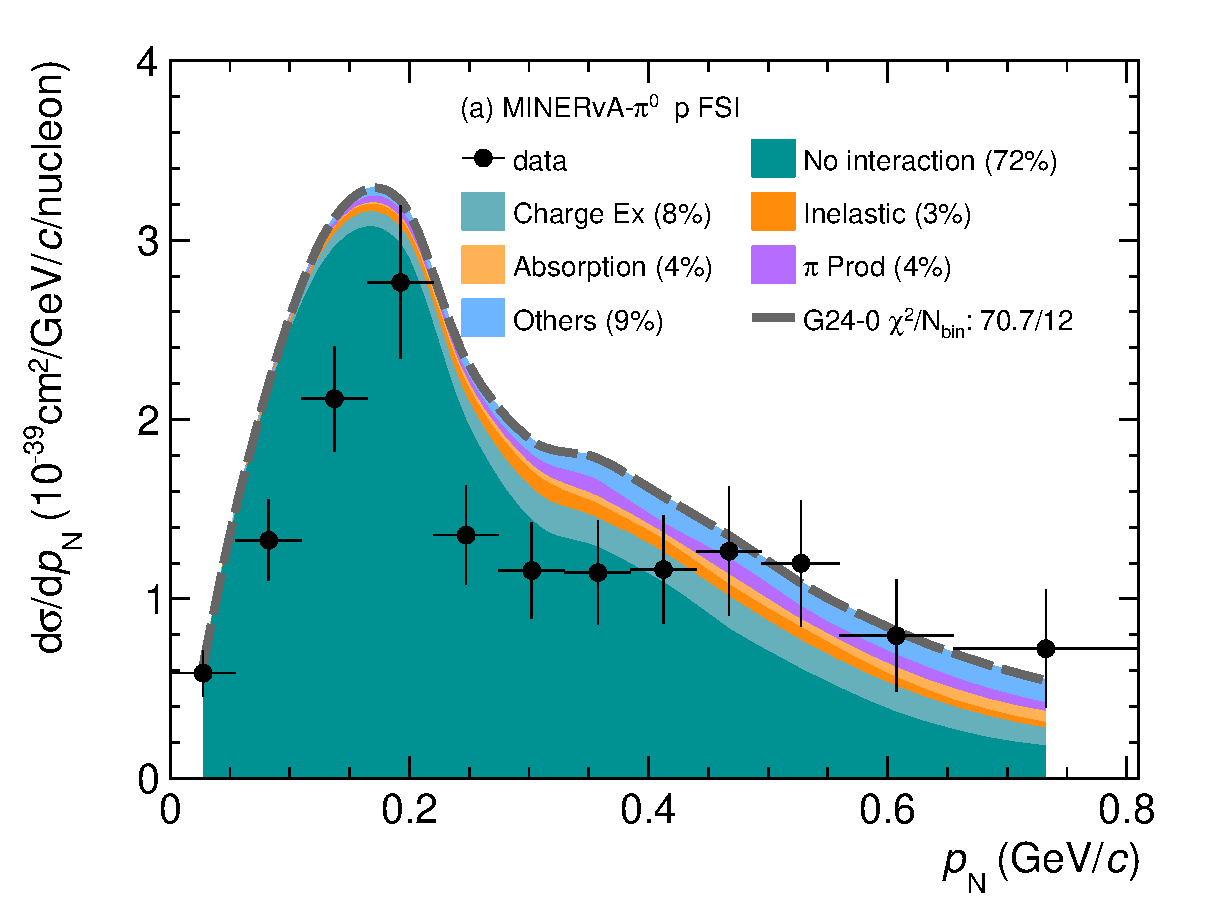
\includegraphics[width=\dbfigwid\textwidth]{figures/tuning/0000-min_pi0_pn_pr_decomp_cex.eps}
        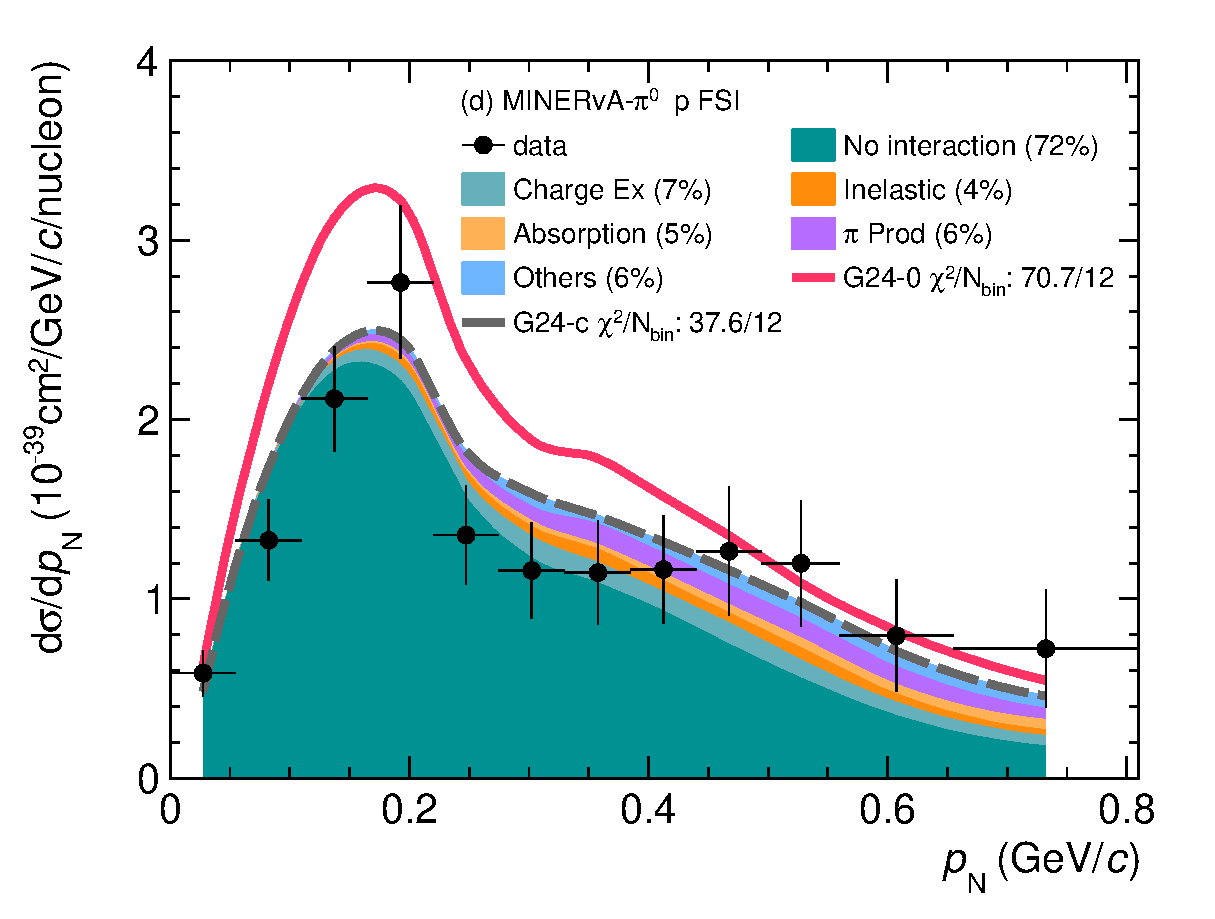
\includegraphics[width=\dbfigwid\textwidth]{figures/tuning/0026-min_pi0_pn_pr_decomp_covfix.eps}	
        \caption{\label{fig:minpiz-pn-pr} Similar to Fig.~\ref{fig:CEX-minpiz-dat-pi0} but for $\pn$ with proton FSI fate decomposition. Note that the ``Absorption'' of the proton is referring to the absorption of the $\pip$ from the decay of $\deltapp$, which could lead to emission of nucleons as discussed in Sec.~\ref{sec:tuning-para-choice}.     
        } 
    \end{figure}

    Although the interaction models (e.g., 2p2h) are not tuned explicitly, their fractional contributions show modest adjustments in Fig.~\ref{fig:g24-c-dat-reac} and Fig.~\ref{fig:g24-c-pn-reac} compared to Fig.~\ref{fig:g24-0-dat-reac} and Fig.~\ref{fig:g24-0-pn-reac}. 
    This change is driven by the increased $\srcfr$, which results in a higher number of events with elevated initial nucleon momenta, thereby enhancing interactions that require greater initial state energy, such as RES and DIS. 
    For example, the RES component rises from $19\%$ in Fig.~\ref{fig:g24-0-pn-reac}c to $24\%$ in Fig.~\ref{fig:g24-c-pn-reac}c for \minzpi. 
    Consequently, the relative contributions of the other interactions are slightly reduced; in particular, the 2p2h fraction decreases from $31\%$ to $30\%$ for \minzpi.

\section{Discussion}
Among the 26 observable combinations considered for the \allpar\ and \redpar\ tunes, combination \cbRedPar\ in the \redpar\ tune yields the best result.
This result offers valuable insights for future tuning efforts—both the selection of observables and the choice of parameters are critical for a successful tuning.
Increasing the number of parameters and observables does not necessarily improve the outcome.
Instead, it is preferable to include only those parameters that significantly affect the selected observables and only those observables that are highly sensitive to the chosen parameters while exhibiting minimal dependence on others.
For example, $\dphit$ is excluded from \cbRedPar\ because it is strongly influenced by the neutrino energy, which is not modified by any of the tuning parameters.
Admittedly, practical limitations in our understanding of the model and the data can preclude this ideal.
Nevertheless, optimizing the sensitivity matching between observables and model parameters is essential for achieving the best results.

The \gC\ fit results imply extreme parameter values, yet their impact on observables is less pronounced than the magnitude of the parameter changes might suggest. 
For individual FSI fate cross sections, the renormalization applied after scaling causes the effective change for a given fate to be smaller than the scaling parameter alone, as detailed in Sec.~\ref{sec:tuning-para-choice}.
Regarding the total FSI cross sections, only that of $\piz$ is altered.
Figure~\ref{fig:pizmfp_change} displays the total $\piz$-C scattering cross section as a function of the pion kinetic energy. 
The overall shape remains similar and consistent with Fig. 2.23 (for $\pip$-C reactions) in Ref.~\cite{Andreopoulos:2015wxa}, although the peak increases from $380$ to $489$~mb---a $29\%$ rise---which is significantly less than the scaling factor $\pizmfp=0.34$ might imply. 
Moreover, the default $\piz$ parameter values are derived from charged pion data under the assumption of isospin symmetry rather than being directly extracted from experimental measurements. 
Consequently, this modification does not conflict with existing agreements based on hadron scattering data.
\begin{figure}[!htb] 	
    \centering 		
    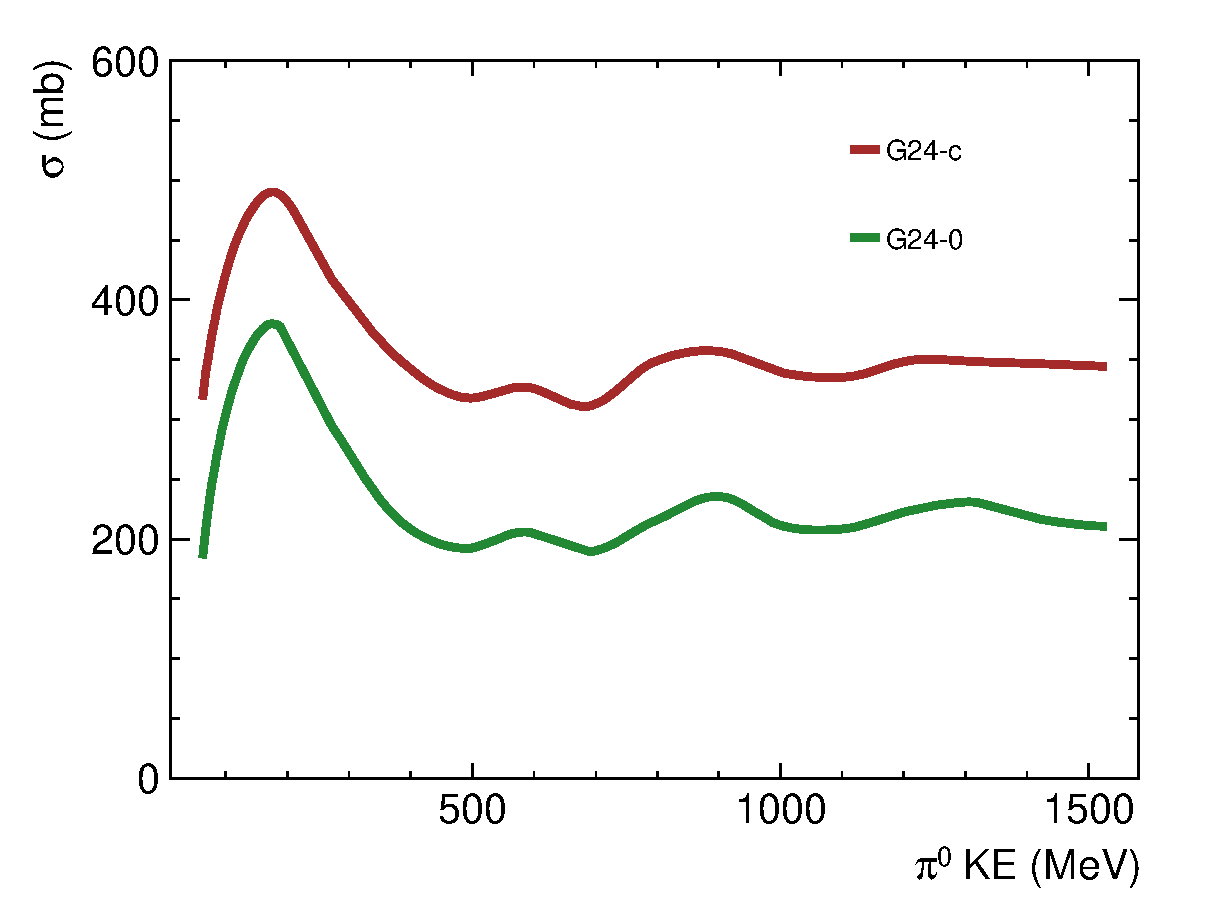
\includegraphics[width=\sgfigwid\textwidth]{figures/tuning/pi0mfp_change_covfix.eps}
    \caption{\label{fig:pizmfp_change} Change in MC prediction for $\piz$ cross section between \gZero\ and \gC. } 
\end{figure}
Furthermore, the overall agreement of this tune with most non-TKI neutrino datasets remains virtually unchanged before and after tuning, thereby corroborating the physicality of the model.

While exclusive electron scattering data would offer excellent constraints on FSI models, most current electron scattering measurements are inclusive~\cite{electronsforneutrinos:2020tbf} and are not ideally suited for FSI tuning.
The ``Electrons for Neutrinos'' (e4nu) collaboration uses data from the CLAS6 spectrometer to measure exclusive final states, such as the $1\textrm{p}0\pi$ cross-section on carbon as a function of TKI variables~\cite{CLAS:2021neh}.
However, in the context of electron-scattering pion production, \genie\ tends to over-predict the data due to the absence of dedicated tunes based on free nucleon data. 
Large uncertainties in the pion production model thus obscure any underlying nuclear or FSI dependence. 
To resolve these effects, one must first tune electron scattering to free nucleon data. 
The current tuning study can be extended in the future when dedicated electron-pion production measurements become available.

In summary, this tune constitutes a valid and effective model that serves as a robust starting point for further analyses. 
Future refinements will be achievable as additional data, including non-TKI observables and electron-scattering measurements, are incorporated into the fit.

\section{\label{sec:summary}Summary and outlook}
This work represents the first global tuning effort on TKI data. 
Our partial tune of the \sfcfg\ and hA models, $\restunefull$ (\gC), yields an effective model that improves the description of both neutrino-hydrocarbon pionless and pion production interactions. 
The most significant modification in the model is driven by the \minpiz\ TKI measurement~\cite{MINERvA:2020anu}, which was considerably overestimated by \genie\ as shown in Fig.~\ref{fig:g24-0-dat-reac}d and Fig.~\ref{fig:g24-0-pn-reac}d. 
This improvement is crucial for the next generation of precision GeV neutrino experiments. 
This tuning configuration has been integrated into the \texttt{master} branch of \genie\ and is scheduled for inclusion in the upcoming release.

To develop an effective model, we concentrated on the parameters most sensitive to the data, namely $\srcfr$, $\pizmfp$, $\picex$, $\ncex$, $\nabs$, and $\npiprod$, thereby reducing the total number of adjustable parameters from 14 to 6. 
The optimal combination of observables comprises $\dat$, $\pn$ (or $\dpt$ when $\pn$ is unavailable), and $\dptt$, drawn from both pionless and pion-production measurements in T2K and MINERvA. 
In this approach, the pion production model remains fixed, so that the tuned values of $\pizmfp$, $\picex$, $\nabs$, and $\npiprod$ diverge from the constraints established by hadron scattering data. 
A different pion production model might partially compensate for these tuning effects~\cite{Yan:2024kkg}. 
We also opted for the hA FSI model due to its simplicity and numerical efficiency, as noted in Ref.~\cite{GENIE:2022qrc}.
Future studies might consider more sophisticated alternatives. 
With the current set of four TKI measurements from T2K and MINERvA, alternative effective tunes, such as $\alttune$ (\gT\), have also been derived. 
The degeneracy among these tunes can be resolved with additional data, particularly from argon-based measurements~\cite{MicroBooNE:2022emb, MicroBooNE:2023cmw, MicroBooNE:2023tzj, MicroBooNE:2023wzy, MicroBooNE:2024tmp, MicroBooNE:2015bmn} and e4nu experiments~\cite{CLAS:2021neh}.

%========= old ===================
% The GENIE collaboration has demonstrated successful tuning of the various components of the neutrino-nucleus interaction model. 
% For instance, 

% The large data samples and superb imaging capabilities of modern neutrino experiments offer us a detailed new look at neutrino interaction physics. 
% Recently, the GENIE~\cite{Andreopoulos:2009rq, GENIE:2021npt} Collaboration has made substantial progress towards a global tuning using neutrino, charged lepton, and hadron scattering data, in an attempt to integrate new experimental constraints with state-of-the-art theories and construct robust and comprehensive simulations of neutrino interactions with matter. 
% Cross-experiment and cross-topology analyses are challenging tasks as each measurement features its unique selection criteria and various other aspects, such as the neutrino flux. 
% \genie\ has built an advanced tuning framework that enables the validation and tuning of comprehensive interaction models using an extensive curated database of measurements of neutrino, charged lepton, and hadron scattering off nucleus and nuclei. 
% So far, the non-resonant backgrounds~\cite{GENIE:2021zuu}, hadronization~\cite{GENIE:2021wox}, and the quasielastic (QE) and 2-particle-2-hole (2p2h) components~\cite{GENIE:2022qrc} of the neutrino-nucleus interaction have been tuned with $\nu_\mu$ and $\bar{\nu}_\mu$ charged-current (CC) pionless (0$\pi$) data from MiniBooNE, T2K, and MINERvA. 
% A partial tune was performed for each experiment, highlighting the neutrino energy dependence on the QE and 2p2h tuned cross sections. 
% Even though post-tune predictions enhanced the data description for each experiment, the added degrees of freedom were not sufficient to fully describe all CC0$\pi$ data and exhibited tensions with some proton observables~\cite{GENIE:2022qrc}. 
% More exclusive measurements result in additional model constraints. 
% In addition, observables that are sensitive to targeted aspects of the complex dynamics of neutrino interactions are invaluable for model tuning. 
% The transverse kinematic imbalance (TKI)~\cite{Lu:2015hea, Lu:2015tcr}, a final-state correlation between the CC lepton and the hadronic system, is a good example since it is sensitive to the initial-state nuclear environment and hadronic FSI. 
% Our next step is to incorporate TKI data from experiments where various exclusive topologies at different energies are considered. 
% This marks the first combined tuning on TKI data with and without pions in the final states and serves as the starting point of a more comprehensive tuning effort in the energy region most relevant for future accelerator-based neutrino experiments.  

% This chapter is structured as follows: 
% Sec.~\ref{sec:genie} reviews the \genie\ models, and Sec.~\ref{sec:Tuning} details the tuning considerations and procedures. 
% Results are summarized in Sec.~\ref{sec:results}, highlighting how the data-MC discrepancy in the \minpiz\ TKI measurement~\cite{MINERvA:2020anu} is resolved while maintaining good data-MC agreement elsewhere. 
% The last section summarises the chapter and outlines future work.

% The definitions of the kinematic cuts for these samples are summarized in Table~\ref{tab:fit-var-combo-phase-space-cut}. 

% \section{\genie\ Model Selection and Configuration}\label{sec:genie}
% \subsection{\label{sec:tuning-obs-choice} Data points}
% \section{\label{sec:results}The first TKI-driven \genie\ tunes}
%========= old ===================
